\documentclass[english, a4paper]{article}

\usepackage[T1]{fontenc}    % Riktig fontencoding
\usepackage[utf8]{inputenc} % Riktig tegnsett
\usepackage{babel}   % Ordelingsregler, osv
\usepackage{graphicx}       % Inkludere bilder
\usepackage{booktabs}       % Ordentlige tabeller
\usepackage{url}            % Skrive url-er
\usepackage{textcomp}       % Den greske bokstaven micro i text-mode
\usepackage{units}          % Skrive enheter riktig
\usepackage{float}          % Figurer dukker opp der du ber om
\usepackage{lipsum}         % Blindtekst
\usepackage{subcaption} 
\usepackage{amssymb}
\usepackage{color}
\usepackage{amsmath}  
\usepackage{amsthm}
\usepackage{braket} 
\usepackage{multicol}
%\usepackage[]{mcode}

% add source code in box
\usepackage{xcolor}
\usepackage{listings}
\usepackage{caption}
\DeclareCaptionFont{white}{\color{white}}
\DeclareCaptionFormat{listing}{%
  \parbox{\textwidth}{\colorbox{gray}{\parbox{\textwidth}{#1#2#3}}\vskip-4pt}}
\captionsetup[lstlisting]{format=listing,labelfont=white,textfont=white}
\lstset{frame=lrb,xleftmargin=\fboxsep,xrightmargin=-\fboxsep}

\usepackage{amsfonts}
\usepackage{setspace}
\usepackage[cm]{fullpage}		% Smalere marger.
\usepackage{verbatim} % kommentarfelt.
\setlength{\columnseprule}{1pt}	%(width of separationline)
\setlength{\columnsep}{1.0cm}	%(space from separation line)
\newcommand\lr[1]{\left(#1\right)} 
\newcommand\lrb[1]{\left[#1\right]} 
\newcommand\bk[1]{\langle#1\rangle} 
\newcommand\uu[1]{\underline{\underline{#1}}} % Understreker dobbelt.



% JF i margen
\makeatletter
\makeatother
\newcommand{\jf}[1]{\subsubsection*{JF #1}\vspace*{-2\baselineskip}}

% Skru av seksjonsnummerering (-1)
\setcounter{secnumdepth}{3}

\begin{document}

\section{Molecular dynamics}

\subsection{1 Molecular Dynamics algorithms}
\textit{Discuss the algorithms for molecular dynamics modeling: Potentials, integration,
cut-off, periodic boundary conditions, initialization, efficiency improvements.} \\

\noindent
MD-simuleringer er en teknikk for å beregne likevekt- og transportegenskaper til et 
klassisk many-body system. Klassisk betyr at bevegelsen til legemene styres av den klassiske mekanikkens
lover, dvs. Newtons lover. Det er ingen interne tilstander i atomene eller i deres interaksjoner, derfor
vil posisjonene og hastighetene til alle partiklene være en fullstendig beskrivelse av systemet. \\

\noindent
En simulering har følgende steg:
\begin{enumerate}
 \item Lager et system med N partikler i en viss konfigurasjon og med gitte initialhastigheter
 \item Løser Newtons bevegelseslikninger for system til egenskapene ikke forandrer seg i tid lenger, 
 dvs. er i likevekt
 \item Måler diverse egenskaper etter equilibration. Disse egenskapene må følgelig være uttrykt
 ved posisjonene og bevegelsesmengdene til partiklene
\end{enumerate}

\subsubsection{Initialization}
Første steg er å initialisere system, dvs. angi posisjoner og hastigheter.
Vi bruker en krystallstruktur som kalles face-centered cubic (FCC) lattice.
Face-centered betyr at atomene er plassert på \textit{sidene} av en enhetskube, dvs
med ett atom i hvert hjørne pluss et på midten av hver side.
Dette svarer til
krystallstrukturen til Argon. Et lattice beksrives av et sett av basisvektorer $\hat{u}_n, n = 1,2,3$
og hver celle er gitt ved en lineær sum med heltallsfaktorer for hver basisvektor. 
Posisjonene til hver basiscelle i en $N_x \times N_y \times N_z$ lattice er derfor
\begin{equation}
 \vec{R}_{i,j,k} = i\hat{u}_1 + j\hat{u}_2 + k\hat{u}_3
\end{equation}
for $i = 1,2,\dots,N_x$ og tilsvarende for $j$ og $k$. Basisvektorene er kartesiske enhetsvektorer
ganget med latticekonstanten $b$, dvs. lengden av en enhetscelle:
\begin{equation}
 \hat{u}_1 = b\hat{i}, \quad \hat{u}_2 = b\hat{j}, \quad \hat{u}_3 = b\hat{k}
\end{equation}
Posisjonene til atomene i hver celle er gitt relativt til posisjonen til basecellen. 
For FCC er disse relative posisjonene
\begin{equation}
 \vec{r} = 0\hat{i} + 0\hat{j} + 0\hat{k},
\end{equation}
\begin{equation}
 \vec{r} = \frac{b}{2}\hat{i} + \frac{b}{2}\hat{j} + 0\hat{k},
\end{equation}
\begin{equation}
 \vec{r} = 0\hat{i} + \frac{b}{2}\hat{j} + \frac{b}{2}\hat{k},
\end{equation}
\begin{equation}
 \vec{r} = \frac{b}{2}\hat{i} + 0\hat{j} + \frac{b}{2}\hat{k},
\end{equation}
For solid Argon, $b = 5.620$ Å. Det gjøres slik i programmet:
\begin{lstlisting}
Atom *atom1 = new Atom(mass);
atom1->position.set(lc*i, lc*j, lc*k);
atom1->storeInitialPosition();
if (BoltzmannDist) { atom1->resetVelocityMaxwellian(temperature); }
else               { atom1->resetVelocityUniform(maxMinVelocity); }
m_atoms.push_back(atom1);
atom1->setIndex(index);
index++;

Atom *atom2 = new Atom(mass);
atom2->position.set(lc*(i+0.5), lc*(j+0.5), lc*k);
atom2->storeInitialPosition();
if (BoltzmannDist) { atom2->resetVelocityMaxwellian(temperature); }
else               { atom2->resetVelocityUniform(maxMinVelocity); }
m_atoms.push_back(atom2);
atom2->setIndex(index);
index++;
\end{lstlisting}

\noindent
Man kan angi forskjellig type initialhastigheter.
Fra statistisk fysikk vet vi at ved likevekt ved temperatur $T$, er hastighetene til atomene
gitt av Boltzmann-distribusjonen, dvs. at $x$-, $y$- og $z$-komponentene til hastigheten er
normaldistribuert med snitt null og standardavvik $\sqrt{k_BT/m}$, der $m$ er massen til et atom
og $k_B$ er Boltzmann-konstanten. $m = 39.948\,\textrm{a.u.}$ for Argon. $k_B = 1$
for atomic units. \\

\noindent
Man kan også starte med hastigheter som er uniformt distruberte random tall i invervallet $[-v,v]$.
I følge central limit theorem skal hastighetsdistribusjonen til partiklene ende opp i
Maxwell-Boltzmann-distribusjonen uavhengig av hva man starter med. Dette kan være en fin test av koden.

\subsubsection{Integration}
Vi bruker den symplektiske og numerisk stabile Velocity-Verlet-algoritmen for å løse 
Newtons likninger for hvert tidssteg. Denne utvikler posisjonene og hastighetene til alle 
atomene fremover i tid. Symplektisk betyr at vi unngår \textit{energy drift}, dvs. at totalenergien
øker eller minker litt over tid, selv om den egentlig skal være bevart for et lukket system / 
mikrokanonisk ensemble. Energy drift kommer av av tidssteget ikke er uendelig lite.
Med Velocity Verlet vil energien oscillere rundt den eksakte verdien. 
Algoritmen er som følger:
\begin{enumerate}
 \item Finn hastigheten for halve tidssteget fremover: 
 \begin{equation}
  {\bf v}_i(t + \Delta t/2) = {\bf v}_i(t) + \frac{{\bf F}_i(t)}{2m} \Delta t
 \end{equation}
 \item Finn nye posisjoner basert på denne hastigheten:
 \begin{equation}
  {\bf r}_i(t + \Delta t) = {\bf r}_i(t) + {\bf v}_i(t + \Delta t/2)\Delta t
 \end{equation}
 \item Regn ut de nye kreftene på hvert atom basert på de nye posisjonene:
 \begin{equation}
  {\bf F}_i(t + \Delta t) = -\nabla_iU_i({\bf \{r\}}(t + \Delta t))
 \end{equation}
 \item Regn ut de ny hastighetene:
 \begin{equation}
  {\bf v}_i(t + \Delta t) = {\bf v}_i(t+\Delta t/2) + \frac{{\bf F}_i(t + \Delta t)}{2m} \Delta t
 \end{equation}
\end{enumerate}
Hver av disse likningene er utledet ved Euler-metoden. Velocity Verlet har en global feil som 
går som $\mathcal{O}(\Delta t^2)$. 

\subsubsection{Potensial}
Vi ser fra Velocity-Verlet at kreftene på alle atomene bestemmes av et potensial $U$.
Vi bruker her Lennard-Jones-potensialet for å simulere parvis interaksjon:
\begin{equation}
 U(r) = 4\epsilon\left[\left(\frac{\sigma}{r}\right)^{12} - \left(\frac{\sigma}{r}\right)^6 \right]
\end{equation}
Dette potensialet approksimerer interaksjon mellom par av nøytrale atomer. 
$r$ er avstanden mellom partiklene, $\epsilon$ er dybden av potensialbrønnen og $\sigma$ er
avstanden er potensialet er null. Optimale verdier av parametrene for argon:
\begin{equation}
 \frac{\epsilon}{k_B} = 119.8 K, \quad \sigma = 3.405
\end{equation}
$\sigma$ måles i Ångstrøm. Det første leddet er frastøtende, som skyldes overlapping av elektronorbitaler.
Det andre leddet er attraktivt for lengre avstander, skyldes van-der-Waals-krefter (Londonkraft). 
Potensialet ser slik ut:
\begin{figure}[H]
\begin{center}
  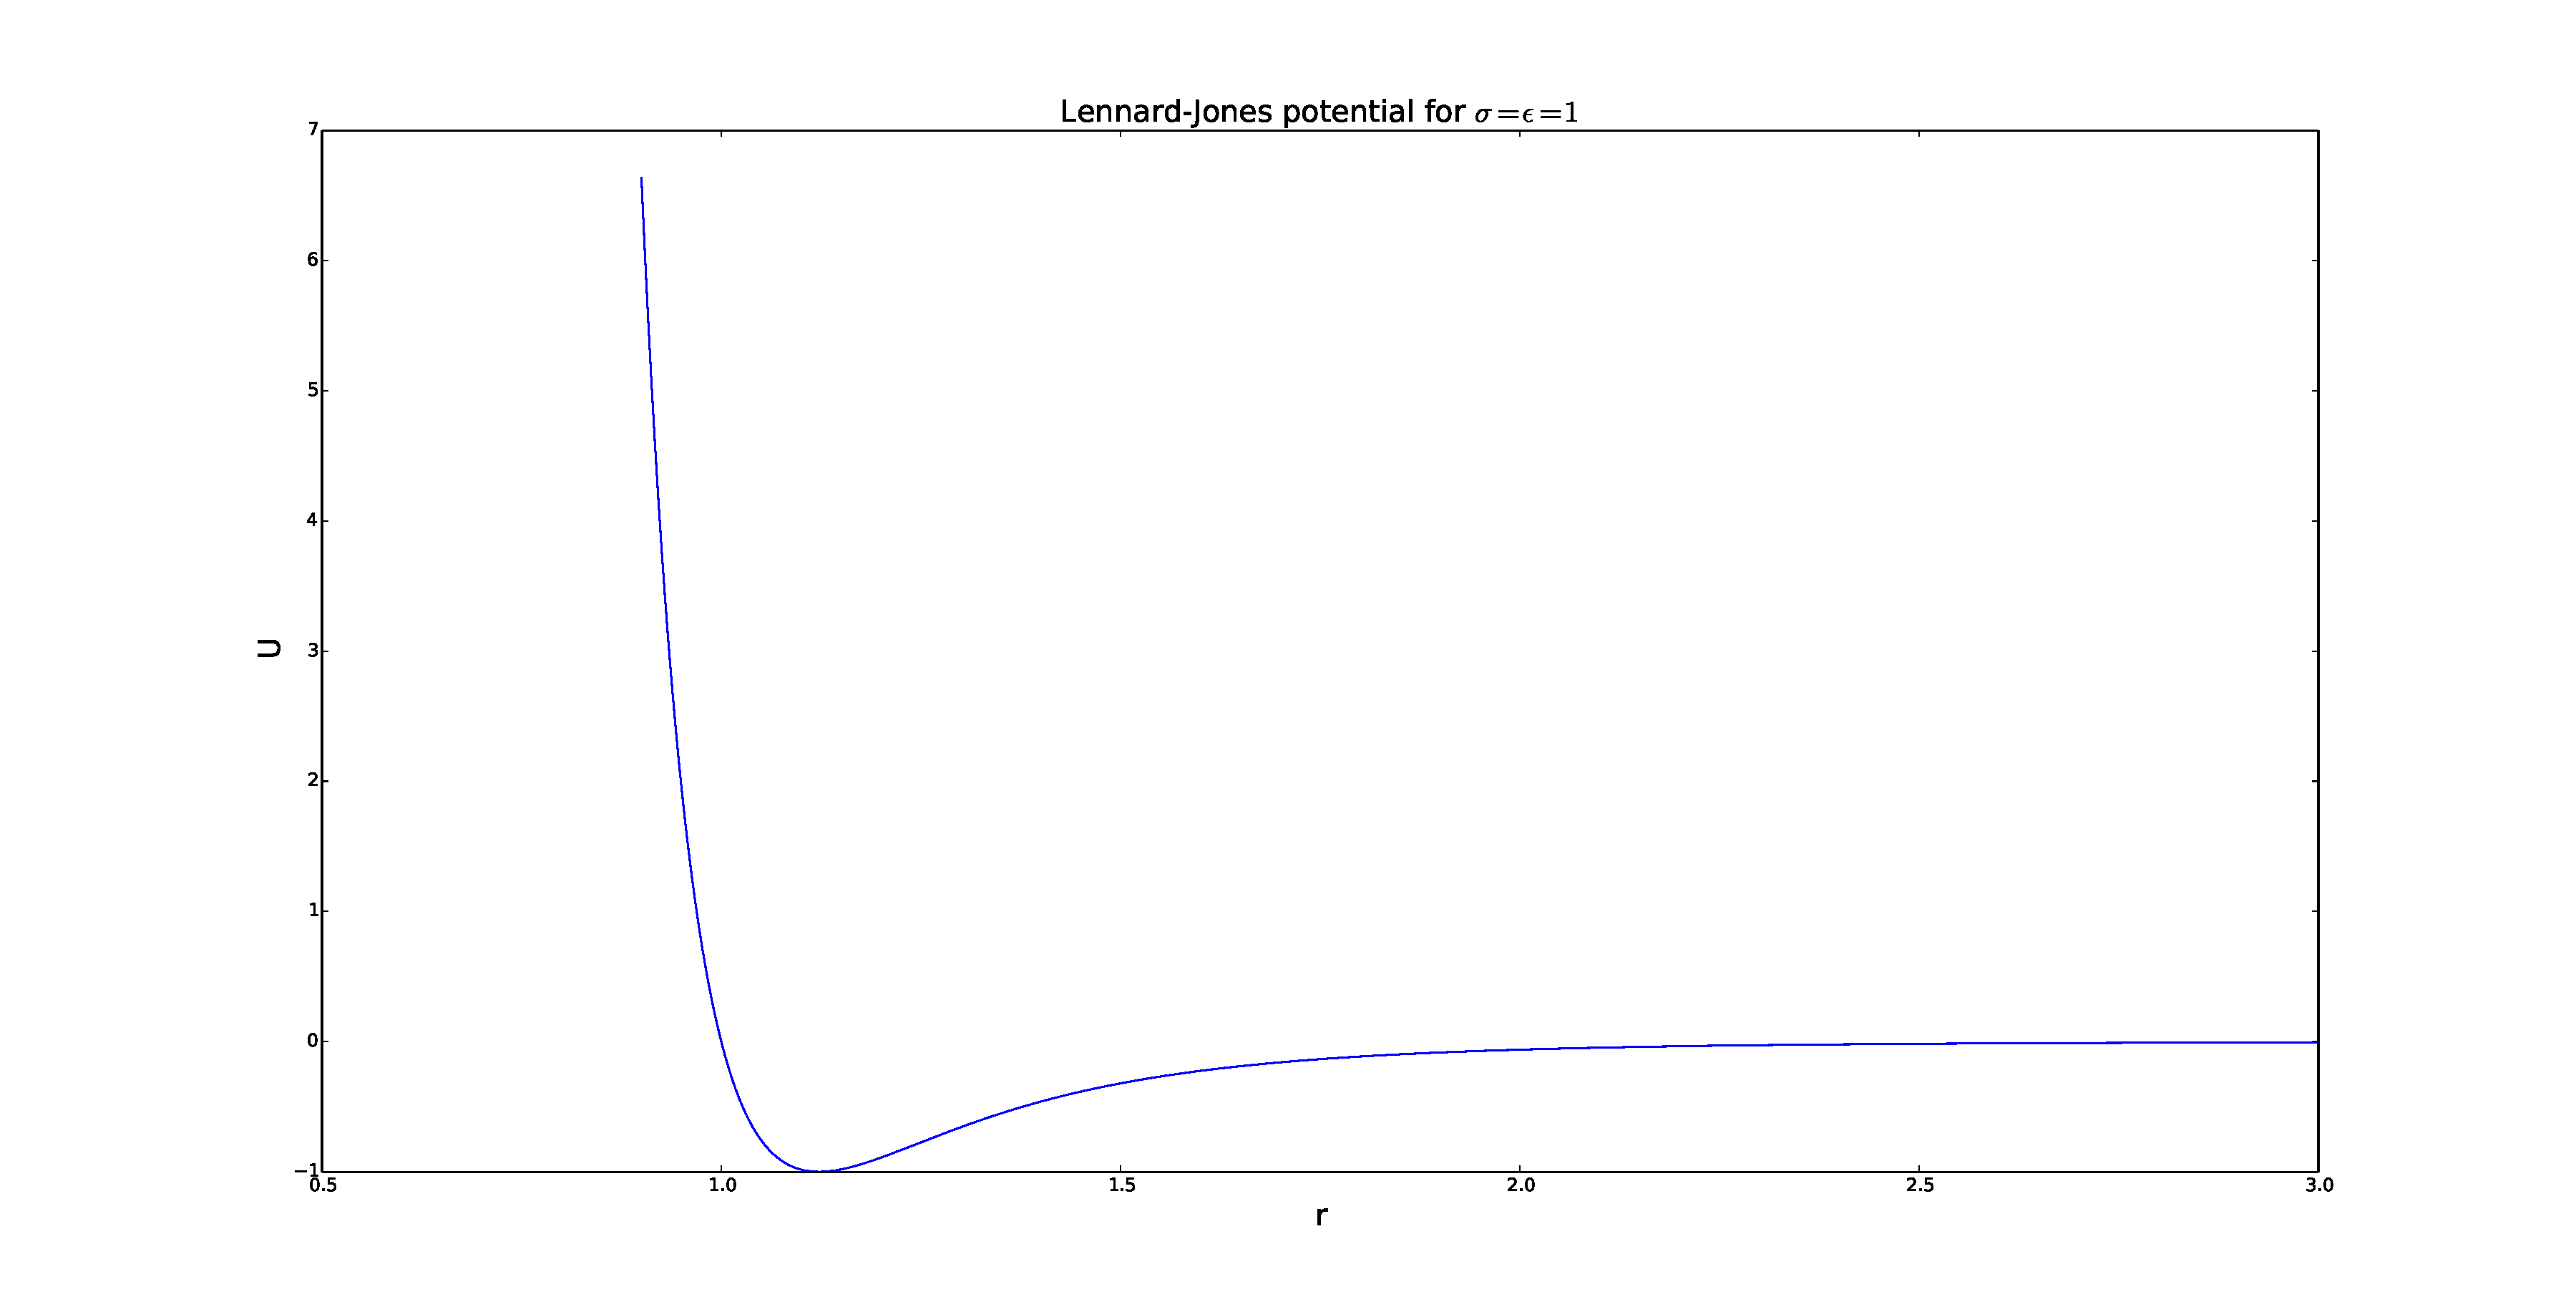
\includegraphics[width = 140mm]{lennard-jones.pdf}
  \caption{Lennard-Jones potential}\label{fig:fig1}
  \end{center}
\end{figure}
Dette er et konservativt potensial (avhenger bare av posisjoner), slik at kraften på atom 
$i$ fra atom $j$ er
\begin{equation}
 {\bf F}_i = -\nabla_i U_i = \frac{24}{r_{ij}^6}\left(\frac{2}{r_{ij}^6} - 1\right)
 \frac{{\bf r}_i - {\bf r}_j}{r_{ij}^2}
\end{equation}
og kraften på atom $j$ fra atom $i$ kan da regnes ut som (i følge Newtons tredje lov):
\begin{equation}
 {\bf F}_i = -{\bf F}_j
\end{equation}
Den totale kraften på atom $i$ er summen av kreftene fra alle de andre partiklene:
\begin{equation}
 {\bf F}_i^{tot} = \sum_{i<j} {\bf F}_j
\end{equation}
der vi bare tar med atomene $j>i$ for å forhindre at kraften på atom $j$ fra atom $i$
adderes to ganger.

\subsubsection{Periodic boundary conditions}
Mange av atomene vil etter hvert bevege seg ut av systemet vårt. Et triks for å simulere et stort
(uendelig) system er å bruke periodiske grensebetingelser. Dvs. at dersom en partikkel forlater systemet 
ved å bevege seg ut av en av sidene av kuben, vil den dukke opp på motsatt side med samme hastighet. 
Dette må gjøres komponentvis. Vårt system er $[0,L] \times [0,L] \times [0,L]$
der $L = bN_c$, $N_c$ er antall unit cells i hver retning. PBC implementeres slik:
\begin{itemize}
 \item For hver posisjonskompononent ${\bf r}_i$:
 \begin{itemize}
  \item if ${\bf r}_i < 0$: ${\bf r}_i = {\bf r}_i + L$
  \item else if ${\bf r}_i > L$: ${\bf r}_i = {\bf r}_i - L$
 \end{itemize}
\end{itemize}
Dette må også tas hensyn til når man regner ut kreftene. Vi bruker \textit{minimum image convention}, dvs.
at avstanden vi velger den korteste avstanden mellom to atomer. Dersom to atomer er nær $x$-veggen på hver sin side, 
er den korteste avstanden ikke den som regnes ut, men den gjennom veggen. Man må dermed legge til eller
trekke fra $L$ for å finne den minste forskjellen. Matematisk:
\begin{equation}
 \textrm{min}_\delta(x_i - x_j + \delta L), \quad \delta \in \{-1,0,1\}
\end{equation}
For å vite om avstanden man har regnet ut er for stor, tester man om den er større enn $L/2$. 
Dette begrenser interaksjonsrekkevidden til $L/2$, som er mer enn nok for vårt potensial, som har 
ganske lav rekkevidde (går som $1/r^6$ og $1/r^{12}$). Implementeres slik:
\begin{itemize}
 \item For hver posisjonskomponent ${\bf r}_i$:
 \begin{itemize}
  \item if $x_{ij} > L/2$: $x_{ij} = x_{ij} - L$
  \item else if $x_{ij} < -L/2$: $x_{ij} = x_{ij} + L$
 \end{itemize}
\end{itemize}

\subsubsection{Efficiency improvements}
Vi kan gjøre enkle ting som å unngå å gange med konstanter i løkker. 
I tillegg bruker vi cellelister og nabolister. Kreftene tar mest tid å regne ut, antall krefter
vi må regne ut er $\frac{1}{2}N(N-1)$ for hvert tidssteg, med en tidsskalering $\mathcal{O}(N^2)$.
L-J-interaksjonen har lav rekkevidde og kan neglisjeres for avstander over $r_{cut} \approx 3\epsilon$.
Dette oppnås ved å dele inn systemet i celler med størrelse $r_{cut}$. Et atom vil kun interagere
med atomene i de 26 nabocellene. Antall celler i hver dimensjon regnes ut slik:
\begin{equation}
 n = L/r_{cut}
\end{equation}
og vi finner ut hvilken celle $(i,j,k)$ hvert atom er i slik:
\begin{equation}
 i = (x/L) \cdot n
\end{equation}
for $x, y, z$. I hver celle $(i,j,k)$ lagres pekere til alle atomobjektene som hører til i denne cellen. 
Vi lager også en naboliste, som er 2-dimensjonal vektor. Element $(i',j')$ i denne vektoren
er nabo $j'$ til atom $i'$. Naboene finnes ved for hver celle å plukke ut indeksene til alle
nabocellene, her må det tas hensyn til PBC. Nabocellene til celle $(i,j,k)$ er alle cellene med indekser
\begin{equation}
 (i',j',k') \in (i + \delta, j + \delta, k + \delta) \quad \delta \in \{-1,0,1\}
\end{equation}
som blir $3^3 - 1  = 26$ naboceller (må trekke fra gjeldene celle). For hvert naboatom
sjekkes det om avstanden er mindre enn $r_{cut}$. Dersom den er det, legges naboatomet til listen 
over naboatomer til det gjeldene atomet. Siden vi opererer med svært korte tidssteg, vil atomene bevege seg
lite for hvert steg. Cellelistene oppdateres derfor kun for hvert tiende steg. 


\subsection{2 Molecular dynamics in the microcanonical ensemble}
\textit{Discuss initialization and initialization effects. Temperature measurements and fluctuations.
Comment on use of thermostats for initialization.} \\

\noindent
Initialisering av posisjoner og hastigheter er diskutert ovenfor. Et FCC lattice er konstruert slik at
det har minimum potensiell energi. Alle andre initielle konfigurasjoner vil ha større potensiell energi. 
Dvs. at når atomene begynner å bevege på seg, vil den potensielle energien øke, og den kinetiske energien
minke, dette fordi totalenergien er bevart i et mikrokanonisk ensemble (system kan ikke utveksle
energi, volum eller partikler med omgivelsene). Dette vil fortsette helt til vi når en bølgedal der den 
potensielle energien er på et maksimum, før det svinger opp igjen og til slutt stabiliserer seg, men med små
fluktuasjoner. Disse fluktuasjonene vil gå mot null når størrelsen på systemet går mot uendelig. \\

Temperatur er i utgangspunktet ikke lett å måle, men hvis vi antar at det er likevekt mellom
translasjonell og potensielle frihetsgrader, sier ekvipartisjonsprinsippet at hver
kvadratisk frihetsgrad i Hamiltonian for systemet har en gj.sn. energi $\frac{1}{2}k_BT$. 
Gj.sn. total kinetisk energi i tre dimensjoner blir derfor
\begin{equation}
 \langle E_k \rangle = \frac{3}{2}Nk_BT
\end{equation}
slik at temperaturen kan måles ved hvert tidssteg ved å regne ut kinetisk energi,
temperaturen er da gitt ved
\begin{equation}
 T = \frac{2}{3} \frac{\langle E_k \rangle}{Nk_b}
\end{equation}
Den totale kinetiske energien regnes ut (som vanlig) slik:
\begin{equation}
 E_k = \sum_{i=1}^N \frac{1}{2}m_i|{\bf v}_i|^2
\end{equation}
Siden temperaturen er direkte proporsjonal med den gj.sn. kinetiske energien, vil den først ha
den initielle verdien vi setter, før den raskt minker, for så å stabilisere seg med små fluktuasjoner:
\begin{figure}[H]
\begin{center}
  \includegraphics[width = 140mm]{../../molecular-dynamics-fys3150/figures/temperatureLattice8.pdf}
  \caption{Temperature as function of time}\label{fig:fig2}
  \end{center}
\end{figure}
Den faktiske temperaturen vil være gj.sn. temperatur etter systemet har kommet i likevekt.
Den ergodiske hypotesen sier at et tidssnitt og ensemblesnitt av en variabel er lik for et 
system i likevekt studert over lengre tid. Vi kan derfor måle makroskopiske variabler
ved å sample og snitte fra \textit{ett} system over lengre tid. Dette vil være det samme
som å snitte over et ensemble av systemer. Hvor lengre tid hvor mindre blir
den statistiske feilen.

\noindent
Temperaturfluktuasjonene kan være korrelert dersom tidssteget er for lite. 
Vi kan lage en autokorrelasjonsfunksjon for temperaturfluktuasjonene og finne en ideel $\Delta t$ 
for å få riktig standardavvik på fluktuasjonene. 

\noindent
For å simulere det kanoniske ensemblet bruker vi termostater. Det kanoniske kan utveksle energi
med et tenkt, uendelig varmebad med temperatur $T$. Det vil altså ha konstant temperatur, 
partikkelantall og volum, men ikke konstant energi. Termostatene sørger for at $T$ holder seg
konstant på den initielle verdien. Etter ekvilibrering kan termostaten skrus av, og 
makroskopiske variabler kan måles. Termostatene forklares nedenfor. 

Translasjonell invarians vil si at lineær bevegelsesmengde er bevart. Vi vil derfor 
at initiell total lineær bev.mengde skal være null. Vi må derfor fjerne eventuell
bev.mengde etter initialisering av posisjoner og hastigheter er gjort. Dette gjøres ved å
først regne ut total bev.mengde,
\begin{equation}
 p^{tot} = \sum_{i=1}^N m_i v_i
\end{equation}
for deretter å trekke fra hastigheten som tilsvarer den gj.sn. bev.mengden fra hver partikkel:
\begin{equation}
 \vec{v}_i = \vec{v} - p^{tot} / (m_i N)
\end{equation}




\subsection{3 Molecular dynamics in the microcanonical ensemble 2}
\textit{How to measure macroscopic quantities such as temperature and pressure from a 
molecular dynamics simulation. What challenges do you expect? What can it be used for?} \\

\noindent
Hvordan man måler makroskopiske størrelser i en MD-simulering er forklart i seksjonen ovenfor.\\

\noindent
Trykk kan måles på mange måter. Vi bruker et uttrykk som kommer fra viriale likningen for trykk. 
Gj.sn. trykk er
\begin{equation}
 P = \rho k_BT + \frac{1}{3V} \sum_{i<j} \vec{F}_{ij} \cdot \vec{r}_{ij}
\end{equation}
der $V$ er volumet til system, $\rho = N/V$ er partikkeltettheten. Dette uttrykket 
gjelder kun for det mikrokanoniske ensemblet. Trykket regnes ut i kraft-loopen som skalarproduktet
av kraft og avstandsvektor for hvert partikkelpar. 
Trykket har invers form i forhold til temperaturen:
\begin{figure}[H]
  \begin{center}
  \includegraphics[width = 140mm]{../../molecular-dynamics-fys3150/figures/pressureNc10T100.pdf}
  \caption{Trykk som funksjon av tid. $N_c = 10, T = 100 K$}
  \label{fig:fig3}
  \end{center}
\end{figure}
Det er mer interessant å plotte trykk som funksjon av temperatur:
\begin{figure}[H]
  \begin{center}
  \includegraphics[width = 140mm]{../../molecular-dynamics-fys3150/figures/pressureVsT.pdf}
  \caption{Trykk som funksjon av temperatur}
  \label{fig:fig4}
  \end{center}
\end{figure}
Vi ser at trykket er lineær i $T$, slik som en ideell gass for fixed $N$ og $V$:
\begin{equation}
 PV = NkT
\end{equation}
Vår argongass er ikke ideell, iom. at vi har med interaksjoner mellom atomene. Disse
interaksjonene er imidlertid svake, og vi ser at argongassen er tilnærmet ideel.
van-der-Waals-tilstandslikningen har imidlertid også trykke som er lineær i T:
\begin{equation}
 P = \frac{Nkt}{V-b} - \frac{a}{V^2}
\end{equation}
der $a$ er den gj.sn. tiltrekning mellom partiklene og $b$ er volumet fjernet fra det totale volumet for en partikkel.\\

\noindent
Disse målingene kan brukes til å simulere ekte gasser, væsker og (faste stoffer). 


\subsection{4 Measuring the diffusion constant in a molecular dynamics simulation}
\textit{How to measure the diffusion constant in a molecular dynamics simulation - limitations
and challanges. Compare with methods and results from random walk modeling}\\

\noindent
For å karakterisere transporten i en væske måler vi selvdiffusjonen til et atom, 
dvs. måle posisjonen som en funksjon av tid $\vec{r}_i(t)$. Selvdiffusjon er diffusjon av et stoffs
egne atomer, dvs. at vi ikke har en blanding av stoffer og dermed ingen kjemisk potensial-gradient.
Diffusjonskonstanten
regnes ut fra mean square forflytning av alle atomer:
\begin{equation}
 \langle r^2(t) \rangle = \frac{1}{N}\sum_{i=1}^N (\vec{r}(t) - \vec{r}_{initial})^2
\end{equation}
I følge Einstein-relasjonen kan diffusjonen regnes ut fra stigningstallet til denne størrelsen:
\begin{equation}
 \langle r^2(t) \rangle = 6Dt \quad \textrm{when} \quad t \rightarrow \infty
\end{equation}
Denne formelen kan utledes vha. sannsynlighetsdistribusjonen for random walks, som er 
en normaldistribusjon med snitt null og varians $2dDt$ der $d$ er dimensjonen til systemet. 
Siden snittet er null vil mean square displacement være lik variansen, dvs. fluktuasjonene
rundt den endelige, gj. sn. endelige posisjonen til random walken. 
Vi forventer altså at $\langle r^2(t) \rangle$ skal være lineær med tiden for væskefasen av Argon.
For fast stoff-fasen vil mean square displacement oscillere (latticevibrasjoner).
Vi regner ut mean square displacement basert på posisjonene i xyz-filen som lages ved en kjøring.
Alle posisjonene til alle tider skrives til samme fil, vi looper gjennom denne filen og lagrer alle posisjonene i 
en 2-dimensjonal vektor slik at $\textrm{position}[t][i]$ er posisjonen til atom $i$ ved tidssteg $t$ lagret
som en liste $(x,y,z)$. \\

\noindent
For hvert tidssteg looper vi gjennom alle atomene. Her må vi inkorporere PBC. Vi bruker den samme testen
som i kraftloopen, men nå tester vi ikke avstanden mellom to atomer, men lengden på det forrige steget:
\begin{lstlisting}
     for t in xrange(1, noTimeSteps+1):
        # for each timestep: find displacement of all atoms and sum up

        cumulativeDisplacement = 0.0
        for atom in xrange(totalNumberOfAtoms):

            # current total displacement
            dr = positions[t][atom] - positions[0][atom]

            # previous displacement
            previousStep = positions[t][atom] - positions[t-1][atom]

            # check whether atom has gone through box wall
            for dim in xrange(3):
                # test if atom has moved out of left wall
                if previousStep[dim] > systemSizeHalf: 
                    goneThroughWalls[atom][dim] -= 1	
                # test if atom has moved out of right wall
                elif previousStep[dim] < -systemSizeHalf:
                    goneThroughWalls[atom][dim] += 1
       
            dr += goneThroughWalls[atom]*systemSize
            cumulativeDisplacement += np.inner(dr, dr) 
    
        displacement[t-1] = cumulativeDisplacement
\end{lstlisting}
I tillegg har vi en 3-vektor goneThroughWalls for hvert atom som holder styr på hvor mange ganger
atomet har gått gjennom den høyre/venstre veggen i hver dimensjon. Dvs. at vi forestiller oss
at det er mange identiske systemer side-ved-side. Dersom goneThroughWalls [0, 2 0] f.eks,
har det gjeldende atomet gått gjennom den positive y-veggen 2 ganger, og har altså derfor
beveget seg $2 \cdot$ system-størrelsen + sin egen y-koordinat.\\

\noindent
For væskefase av Argon har vi at $b=5.72$. For $T=1.5$ ser plottet slik ut etter termalisering:
\begin{figure}[H]
  \begin{center}
  \includegraphics[width = 140mm]{../../molecular-dynamics-fys3150/figures/diffusionThermalizedT15.pdf}
  \caption{Mean square displacement som funksjon av tid for $T = 1.5$}
  \label{fig:fig5}
  \end{center}
\end{figure}
Vi ser at kurven er lineær, som forventet. Gjør en linear fit og deler den første koeffisienten på 6
for å finne diffusjonskonstanten D. For fast stoff vil det ikke være noe diffusjon, alle 
atomene står kun og vibrerer rundt sin initielle posisjon. 
Her er et plot av diffusjonskonstant som funksjon av temperatur:
\begin{figure}[H]
  \begin{center}
  \includegraphics[width = 140mm]{../../molecular-dynamics-fys3150/figures/diffVsTemp.pdf}
  \caption{Mean square displacement som funksjon av tid for $T = 1.5$}
  \label{fig:fig5}
  \end{center}
\end{figure}
Vi ser at diffusjonskonstanten øker linært med temperaturen, $D \propto T$. 

\subsection{5 Measuring the radial distribution function in molecular dynamics simulations}
\textit{How can you measure the radial distribution function in a molecular dynamics simulation?
What does it tell? What challenges will you face? Compare the measurement of the radial distribution
function to the measurement of the probability densities for a random walk.}\\

\noindent
Den radielle distribusjonsfunksjonen $g(r)$ karakteriserer den mikroskopiske strukturen til et fluid.
Den er definert som den radielle sannsynligheten for å finne et annet atom i avstand $r$ fra et 
tilfeldig atom, mao. atomtettheten i et sfærisk skall av radius $r$ rundt et atom. 
Normaliseres ved å dele på gj.sn. partikkeltetthet slik at
\begin{equation}
 \lim_{r\to\infty} g(r) = 1
\end{equation}
$g(r)$ måles på denne måten:
\begin{itemize}
 \item Velger et tilfeldig atom
 \item Deler vi opp $r \in (0,L/2]$ i bins ved å dele $L/2$ med antall bins
 \item For hvert tidssteg:
 \begin{itemize}
   \item Looper over alle atomene og finner avstanden til det utvalgte atomet
   \item For hvert atom plasserer vi avstanden i riktig bin 
   \item Deler hver bin på tilsvarende skallvolum for å finne tettheten (normaliserer)
   \item Skriver antall atomer i hver bin til fil for hvert tidssteg
 \end{itemize}
\end{itemize}
Etter dette er gjort leser vi inn filen i python og midler over tid. 
Slik er resultatet for 30 bins:
\begin{figure}[H]
  \begin{center}
  \includegraphics[width = 140mm]{../../molecular-dynamics-fys3150/figures/radialDistBins30.pdf}
  \caption{Radiell distribusjonsfunksjon}
  \label{fig:fig5}
  \end{center}
\end{figure}
Vi ser at $g(r/b)$ der $b$ er latticekonstanten er en periodisk funksjon. Vi har en topper med
intervall ca $b/\sqrt{2}$, som er avstanden mellom to atomer i samme celle i en FCC lattice. 
Mellom disse har vi bunner. Vi ser at for $r < b/\sqrt{2}$ er $g(r)$ null. For større avstander
blir toppene og bunnene mindre fordi skallvolumene blir større. $g(r)$ går mot 1 når
$r \to \infty$, som nevnt ovenfor. Dette er en slags referanseavstand. 
For en perfekt krystall ville disse bunnene og toppene være helt skarpe. 
For en væske ser den slik ut:
\begin{figure}[H]
  \begin{center}
  \includegraphics[width = 140mm]{../../molecular-dynamics-fys3150/figures/radialDistLiquidBins50.pdf}
  \caption{Radiell distribusjonsfunksjon}
  \label{fig:fig5}
  \end{center}
\end{figure}
Vi ser at strukturen er mye mindre regulær, som forventet. 


\subsection{6 Thermostats in molecular dynamics simulations}
\textit{Discuss the microcanonical vs the canonical ensemble in molecular dynamics simulations:
How can we obtain results from a canonical ensemble? Introduce two thermostats, and describe their
behaviour qualitatively. How can you use such a thermostat for rapid initialization of a microcanonical
ensemble?} \\

\noindent
For å simulere et kanonisk ensemble / NVT-ensemble, må vi simulere interaksjoner med et 
ekstern varmebad. Dette gjør at temperaturen, men ikke energien, holder seg konstant. Dette gjøres ved
å bruke termostater, som må oppfylle følgende kriterier:
\begin{itemize}
 \item Holde systemtemperaturen ca. ved varmebadtemperaturen
 \item Sample faserommet som tilsvarer det kanoniske ensemblet (dvs. sørge for 
       at posisjonene og hastighetene til atomene utvikler seg som et kanonisk ensemble)
 \item Evnen til å tune variabler
 \item Dynamikken preserveres
\end{itemize}
Vi bruker to forskjellige termostater, Berendsen og Andersen. 

\subsubsection{Berendsen termostat}
Berendsen fungerer slik at den reskalerer hastighetene til alle atomene med en faktor $\gamma$:
\begin{equation}
 \gamma = \sqrt{1 + \frac{\Delta t}{\tau}\left(\frac{T_{bath}}{T} - 1\right)}
\end{equation}
for hvert tidssteg. $\tau$ er relaxation-tid, dvs. tiden det tar før systemet går tilbake til likevekt.
$\tau = \Delta t$ vil gjøre at temperaturen holder seg nøyaktig konstant, men bør settes til 
10-20 ganger denne verdien. 
Denne formelen har som utgangspunkt at temperaturforandringen er prop. med tempforskjellen mellom system
og bath:
\begin{equation}
 \frac{dT}{dt} = \frac{1}{\tau}(T_0 - T)
\end{equation}
som fører til en eksponentiell nedgang av systemtemperaturen mot badtemperaturen. 
Berendsen klarer
ikke å produsere baner i faserommet som korresponderer til det kanoniske ensemblet pga.
denne skaleringen av hastigheter, men den tillatter temperaturfluktuasjoner når $\tau  > \Delta t$.
Den er god på å holde
temperaturen konstant, tilfredsstiller Fourier'r lov om varmeoverføring. 

\subsubsection{Andersen termostat}
Andersen simulerer kollisjoner mellom atomer i systemet og i varmebadet. Energi blir dermed
utvekslet mellom atomene, det er dette som foregår i virkelige systemer, altså varmeledning.
Atomer som kolliderer
får en ny normalt distribuert hastighet med standardavvik $\sqrt{k_BT_{bath}/m}$. 
Dette gjøres slik for hvert tidssteg:
\begin{itemize}
 \item Loop gjennom alle par av atomer og sjekk om de har kollidert. Vi har kollisjon
       dersom avstanden er mindre enn to ganger radiusen til et Argon-atom.
 \item For hvert kolliderende atom genererer vi et uniformt distribuert tilfeldig tall $p$ mellom 
       0 og 1:
       \begin{itemize}
       \item If $p < \Delta t/\tau$: Atomet får en ny hastighet
       \end{itemize}
\end{itemize}
$\tau$ er her kollisjonstid, og bør ha ca samme verdi som for Berendsen. 
Andersen er god på å ekvilibrere system, men forstyrrer dynamikken i f.eks. lattice-vibrasjoner. 
Kan dermed ikke brukes for å måle tidsavhengige størrelser som diffusjon.
Derimot reproduserer Andersen det kanoniske ensemblet eksakt. \\

\noindent
Vi sammenlikner temperaturen som funksjon av tid for de to termostatene:
\begin{figure}[H]
\begin{minipage}[t]{0.48\linewidth}
  \includegraphics[width=\textwidth]{../../molecular-dynamics-fys3150/figures/tempGasBerendsen.pdf}
  \caption{Temperatur som funksjon av tid, Berendsen termostat}
  \label{fig:minipage1}
\end{minipage}
\quad
\begin{minipage}[t]{0.48\linewidth}
\includegraphics[width=\textwidth]{../../molecular-dynamics-fys3150/figures/tempGasAndersen.pdf}
  \caption{Temperatur som funksjon av tid, Andersen termostat}
  \label{fig:minipage1}
\end{minipage}
\end{figure}
Vi ser at Andersen ekvilibrerer raskere, Berendsen derimot har en stor dupp i starten. 
Imidlertid er temperaturfluktuasjonene mindre for Berendsen (men vet ikke hvor store 
fluktuasjonene bør være).
Energiene ser slik ut:
\begin{figure}[H]
\begin{minipage}[t]{0.48\linewidth}
  \includegraphics[width=\textwidth]{../../molecular-dynamics-fys3150/figures/energyGasBerendsen.pdf}
  \caption{Energier som funksjon av tid, Berendsen termostat}
  \label{fig:minipage2}
\end{minipage}
\quad
\begin{minipage}[t]{0.48\linewidth}
\includegraphics[width=\textwidth]{../../molecular-dynamics-fys3150/figures/ernergyGasAndersen.pdf}
  \caption{Energier som funksjon av tid, Andersen termostat}
  \label{fig:minipage2}
\end{minipage}
\end{figure}
Berendsen-termostaten gjør at partiklene beveger seg lenger translasjonelt. Andersen derimot, 
gjør at systemet oppfører seg mer som et fast stoff, med raske, små latticevibrasjoner. 


\section{Advanced molecular dynamics}

\subsection{ 7 Generating a nanoporous material}
\textit{Discuss how we prepare a nanoporous matrix with a given porosity. How do we 
characterize the structure of such a material and the dynamics of a fluid in such a 
material?} \\

\noindent
Et nanoporøst materiale består av to deler: porer og solid materiale. Vi lager et nanoporøst materiale
basert på et allerede termalisert Lennard-Jones-fluid ved å kutte ut deler av systemet. Dette er porene som vi
fyller med fluidet. Inne i porene beveger atomene seg, alle atomer utenfor porene beveger seg ikke, men 
de virker på de bevegende partiklene med krefter. Vi genererer et nanoporøst materiale slik:
\begin{itemize}
 \item Lag en Lennard-Jones-væske med temperatur $T = 0.851$. 
 \item Termaliser væsken
 \item Skru av termalisering, og la programmet kjøre en stund
 \item Lag porer basert på denne termaliserte væsken ved å markere visse atomer som ikke-bevegende
 \item Termaliser evt på nytt
 \item Gjør målinger
\end{itemize}
Porene kan lages på mange forskjellige måter. Man kan f.eks. kutte ut en sylinder som går tvers gjennom
system, som væsken kan bevege seg gjennom. For å lage en sylinder med $r =2$ nm i $x$-retning i midten av system, 
looper vi gjennom alle atomene og regner ut yz-avstanden fra systemSizeHalf. Dersom denne avstanden
er større en sylinderradiusen, merker vi atomet som ikke-bevegende. Disse får da et annet navn enn
Argon-atomene, slik at de får forskjellig farge når vi visualiserer med VMD. Implementeres slik:
\begin{lstlisting}
for (Atom *atom : m_system->atoms()) {
    double yFromCenter = atom->position.y() - m_system->systemSizeHalf().y();
    double zFromCenter = atom->position.z() - m_system->systemSizeHalf().z();
    double distanceFromCenter = yFromCenter*yFromCenter + zFromCenter*zFromCenter;

    if (distanceFromCenter > m_poreRadius) {
	atom->setMovingAtom(false);
	atom->setName("NM");
    }
}
\end{lstlisting}
Hovedmetoden vi skal bruke er å lage porer ved å sette opp flere tilfeldige posisjonerte,
muligens overlappende kuler
med tilfeldige radiuser. Vi gjør slik at matrisen er i kulene, dvs. de ikke-bevegende atomene. 
Væsken er derfor alle atomer utenfor kulene. Vi lager tjue kuler tilfeldig posisjonert med
radiuser uniformt distribuert mellom $R_0 = 2$ nm og $R_1 = 3$ nm. Dette gjøres slik:
\begin{lstlisting}
  for (int i=0; i < m_numberOfPores; i++) {

      // center of random sphere
      vec3 sphereCenter;
      sphereCenter[0] = Random::nextDouble()*m_system->systemSize().x();
      sphereCenter[1] = Random::nextDouble()*m_system->systemSize().y();
      sphereCenter[2] = Random::nextDouble()*m_system->systemSize().z();

      // random radius 2nm-3nm
      double sphereRadius = m_radius0 + Random::nextDouble()*(m_radius1 - m_radius0);
      std::cout << sphereRadius << std::endl;

      // freeze all atoms inside sphere
      for (Atom *atom : m_system->atoms()) {
	  vec3 dr = atom->position - sphereCenter;
	  double distanceFromCenter = dr.length();

	  if (distanceFromCenter < sphereRadius) {
	      std::cout << "yes" << std::endl;
	      atom->setMovingAtom(false);
	      atom->setName("NM");
	  }
      }
  }
\end{lstlisting}
Altså looper vi gjennom alle atomene for hver random pore vi lager og sjekker om de er inni denne eller ikke. 
I så fall merkes de som ikke-bevegende. 

\subsubsection{Porosity}
Porositet er definert som andel volum av systemet som er porer:
\begin{equation}
 \Phi = \frac{V_{pores}}{V}
\end{equation}
Porositet kan måles ved å dele antall bevegende partikler på totalt antall partikler fordi
systemet er relativt homogent. Å sammenlikne antall partikler i porene med totalt antall
partikler blir derfor ekvivalent fordi vi ikke har noen store tetthetsvariasjoner.
\begin{equation}
 \Phi = \frac{N_{moving}}{N}
\end{equation}
Det er vanskelig å avgjøre hva porøsiteten vil bli når vi bruker kulene, dette fordi de overlapper
i varierende grad. Med sylinderen er det derimot enkelt siden vi vet radiusen og volumet til hele
system. Porøsiteten med sylinderen blir
\begin{equation}
 \Phi = \frac{\pi r^2 L}{L^3} = \frac{\pi r^2}{L^2}
\end{equation}
Dersom kulene ikke hadde vært overlappende ville porøsiteten blitt
\begin{equation}
 \Phi = \frac{4}{3}\pi r^3 / L^3
\end{equation}
som ville gitt $\Phi \approx 0.9$ for $b=5.72$ og $N_c = 20$. Altså gjør det faktum at de overlapper
at porøsiteten ca. halveres, den er nemlig ca. 0.5 når kulene overlapper for de samme parametrene.


\subsubsection{Fluiddynamikk}
Væskestrømningen i et nanoporøst materiale kan karakteriseres ved hastighetsprofilen, $u(z)$, 
altså hastighet som funksjon av avstand fra sentrum av en (i dette tilfellet) boks. 
Dersom vi antar at væsken strømmer i $x$-retning pga. en trykkgradient, dvs. en trykkforskjell
fra den ene siden av boksen i forhold til den andre, blir hastigheten en funksjon av $z$. Trykket varierer
kun i $x$-retning. Vi forventer at væsken strømmer raskest i midten av flaten og går mot null
ved kantene. Vi antar to ting om væskestrømmen:
\begin{enumerate}
 \item Non-slip grensebetingelser: Hastigheten til væsken er null ved kantene av porene
 \item Newtonsk væske:
 \begin{equation}
  \sigma_{zx} = \mu \frac{du_z}{dz}
 \end{equation}
 der $\sigma$ er \textit{drag}, dvs. en kraft som virker i motsatt retning av et objekt som beveger seg i 
 en væske. Denne kraften er proporsjonal med viskositeten $\mu$, dvs. en væskes evne til å motstå
 derformasjon, eller tykkelsen til væsken og den deriverte av væskens hastighet i $z$-retning, altså
 når væsken strømmer i $x$-retning. Dragen har både en parallell komponent $x$ og en normal komponent $z$.
\end{enumerate}
Drag er også mellom forskjellige deler av væsken ved laminær strømning, f.eks. vil en partikkel
mer mot midten av flaten strømme fortere, men bli bremset opp av partikler som strømmer parallelt med
denne lenger ut mot sidene. Ut fra dette kan vi utlede hastighetsprofilen:
\begin{equation}
 u(z) = \frac{\Delta p}{L}\frac{1}{2\mu} (a^2 - z)^2
\end{equation}
der $L$ er lengden til systemet i $x$-retning, og $a$ er halve lengden av flaten i $z$-retning. 
Dette er altså en parabel som er null for $z = \pm a$ og maks for $z=0$. Den ser slik ut:
\begin{figure}[H]
  \begin{center}
  \includegraphics[width = 140mm]{../../molecular-dynamics-fys3150/figures/flowProfileSimplePlot.pdf}
  \caption{Strømningsprofil for strømning i $x$-retning}
  \label{fig:fig6}
  \end{center}
\end{figure}
Fluks $Q$, dvs. volum som strømmer gjennom et tverrsnittsareal per tidssteg, er
\begin{equation}
 Q = \frac{2a^3}{3\mu} \frac{\Delta p}{L}
\end{equation}
For et sylindrisk rør er tilsvarende resultater
\begin{equation}
 u(r) = \frac{\Delta p}{L} \frac{1}{4\mu} (a^2 - r^2)
\end{equation}
og
\begin{equation}
 Q = \frac{\pi a^4}{8\mu} \frac{\Delta p}{L}
\end{equation}
Generelt har vi Darcys lov for strømning i et porøst medium:
\begin{equation}
 v_s = \frac{Q}{A} = \frac{k}{\mu}\frac{\Delta p}{L}
 \label{DarcysLaw}
\end{equation}
der $K = k/\mu$ tilsvarer konduktiviteten til mediet, som består av to størrese. $k$ er permeabiliteten, til systemet,
dvs. systemets evne til strømning gjennom seg. 
$v_s$ kalles overfladisk væskestrømhastighet, og er gitt som volumfluksen $Q$ delt på tverrsnittareaelet
$A$ væsken strømmer gjennom. 
Det er ingen direkte sammenheng mellom porøsitet $\Phi$ og permeabilitet $k$. Man kan ha høy $\Phi$, men likevel
lav permeabilitet $k$ dersom det ikke er en pore som går gjennom hele systemet f.eks. Permeabiliteten
sier noe om selve det porøse mediet, mens viskositeten $\mu$ sier noe om væsken. \\



\subsection{8 Diffusion in a nanoporous material}
\textit{How can you measure the diffusion constant for a low-density fluid in a nanoporous system?
Discuss what results you expect. Compare with diffusion in a bulk liquid and in a larger-scale porous
medium}\\

\noindent
Vi kan lage et fluid med halve tettheten ved å loope gjennom alle atomene som beveger seg, og
fjerne annethvert atom:
\begin{lstlisting}
     // remove half of the fluid atoms
    bool everySecondAtom = true;
    for (int i=0; i < m_system->atoms().size(); i++) {
        if (m_system->atoms()[i]->movingAtom()) {
            if (everySecondAtom) {
                m_system->removeAtom(i);
                i--;
                everySecondAtom = false;
            }
            else {
                everySecondAtom = true;
            }
        }
    }
\end{lstlisting}
Vi kan deretter måle diffusjonskonstanten på nøyaktig samme måte som før. Nå derimot, så preparerer
jeg et LJ-fluid med $N_c = 20$ og $T = 1.5$ som jeg termaliserer med Berendsen-termostaten i 1000 tidssteg.
Den siste state-filen leser jeg så inn fra fil, dette er min nye initial state. Når filen er lest inn 
lager jeg kuleporene, og fjerner halvparten av de bevegende atomene. Deretter termaliserer jeg i 501
tidssteg, før jeg kjører uten termostat i 1000 tidssteg til. Her er resultatet:
\begin{figure}[H]
  \begin{center}
  \includegraphics[width = 140mm]{../../molecular-dynamics-fys3150/figures/diffusionSpheresT15.pdf}
  \caption{Diffusjon for kulenanoporøst system for $T=1.5$}
  \label{fig:fig7}
  \end{center}
\end{figure}
Vi ser at $D$ er større enn det ikke-porøse system, noe som er naturlig siden vi har lavere tetthet, som 
fører til at atomene har mer plass til å bevege seg, de blir mindre påvirket av krefter fra andre atomer. 
Dersom tettheten hadde vært den samme derimot, så ville $D$ vært mindre fordi bevegelsen til atomene 
er begrenset av den solide matrisen. 
Også her er $\langle r^2(t) \rangle$ lineær i tid, og vi kan finne $D$ på samme måte. Vi må her huske på
å kun se på diffusjonen til partiklene som beveger seg. \\

\noindent
Et større nanoporøst system kan være et perkolasjonssystem. Her avhenger diffusjon av $p$. 
Dersom vi har $p < p_c$ vil partiklene begrenses av clusterstørrelsen, som vil være liten 
i forhold til systemstørrelsen $L$. Når $p \to p_c$ vil den typiske clusterstørrelsen gå mot uendelig 
(i teorien), men i et endelig system vil den typiske clusterstørrelsen være av størrelse $L$. 
Når $p$ nærmer seg 1 vil så og si alle sites være okkupert, og vi vil få en oppførsel lik 
en bulk (vanlig) væske. 



\subsection{9 Flow in a nanoporous material}
\textit{Discuss how to induce flow in a nanoporous material. How can you check your model,
calculate the fluid viscosity and measure the permeability? What challanges do you expect?} \\

\noindent
For å indusere strømning trenger vi en trykkforskjell over materialet. Dette oppnår vi ved å
introdusere en ekstern kraft $\vec{F} = F_x\hat{i}$ som virker på hvert atom. 
Dette tilsvarer gravitasjon, bare mye sterkere. Denne kraften legges til på hvert atom
i tillegg til de ordinære kreftene i kraft-loopen. Volumfluksen er gitt ved Darcys lov \eqref{DarcysLaw}, 
som også kan skrives
\begin{equation}
 U = \frac{k}{\mu} (\nabla P - \rho g)
\end{equation}
der $\rho$ er massetettheten til fluidet og $g$ er gravitasjonell akselerasjon. 
Denne likningen gjelder for isotropisk porøst medium. Målingene vi gjør må derfor gjøes når systemet
har nådd en stationary state. Vi vet at
\begin{equation}
 \rho g = \frac{M}{V} \frac{F_x}{m} = \frac{Nm}{V}\frac{F_x}{m} = \frac{N}{V}F_x = nF_x
\end{equation}
der $M$ er atomenes totale masse og $n$ er antalltettheten av atomer som kraften $F_x$ virker på. 
Vi har allerede sett at denne loven for en sylinder med radius $a$ er
\begin{equation}
  u(r) = \frac{\Delta p}{L} \frac{1}{4\mu} (a^2 - r^2)
\end{equation}
der $r$ er avstanden fra sylinderens sentrum. Trykkeforskjellen $\Delta p$ kan tilnærmes
som hydrostatisk trykk, dersom vi antar at at væsken er inkompressibel:
\begin{equation}
 \Delta p = \rho gh = nFL
\end{equation}
altså har vi at
\begin{equation}
 u(r) = \frac{nF}{4\mu}(a^2 - r^2)
\end{equation}
Hvis vi nå måler $u(r)$ kan vi regne ut viskositeten $\mu$ ved å finne prop.konstanten til denne likningen, dvs.
gjøre en fit. 
Darcys lov for porøst medium \eqref{DarcysLaw}
er altså
\begin{equation}
 v_s = \frac{Q}{A} = \frac{k}{\mu}\frac{\Delta p}{L} = \frac{k}{\mu}\frac{nFL}{L} = \frac{k}{\mu}nF
\end{equation}
slik at $k$ kan beregnes ved følgende likning
\begin{equation}
 k = \frac{\mu v_s}{nF}  = \frac{\mu}{nF}\frac{Q}{A}
\end{equation}
Vi har her to valg: Enten måle volumstrømningsraten $Q$ eller strømningshastigheten $v_s$. 
Volumstrømningsraten er vanskelig å måle, det måtte i så fall vært partikkelstrømningsrate vi skulle ha målt. 
$v_s$ er gj.sn. strømingshastighet dersom vi antar at væsken strømmer gjennom tomrom, altså enkelfasestrømning. 
Det kan vi anta her, siden væsken strømmer gjennom porer. Altså kan vi måle $v_s$ etter systemet har nådd
en stabil tilstand for å regne ut $k$ etter vi har regnet ut $\mu$. 


\section{Percolation}

\subsection{10 15 Algorithms for percolation systems}
\textit{How do we generate a percolation system for simulations? How to analyze and visualize the systems?
How to find spanning clusters and measure the percolation probability?} \\
\textit{Discuss the behaviour of $\Pi(p,L)$ and $P(p,L)$ in a system with a finite system size $L$. 
How do you measure these quantities?}\\

\noindent
Vi studerer random, porøse medier, dvs. at vi ikke har korrelasjoner i randomness til materialet. 
Vi lager et porøst medium ved å dele materialet inn i kuber (sites) av størrelse $d$. Hver site 
kan være enten fylt eller ikke fylt med materiale. Dersom ikke fylt: pore (tomrom). Hver site
har en sannsynlighet $p$ for å være fylt. Vi genererer et porøst materiale slik:
\begin{lstlisting}
 p = 0.25;
 L = 10;
 z =rand(L,L);
 m = z < p;
 imagesc(m);
\end{lstlisting}
Dette vil generere en $10\times 10$-matrise $m$ der hvert element i matrisen er enten 1 eller 0, dvs. fylt og 
ikke-fylt respektivt. Visualiseres med funksjonen \textit{imagesc}, som fargekoder hver site etter verdier.
\begin{figure}[H]
  \begin{center}
  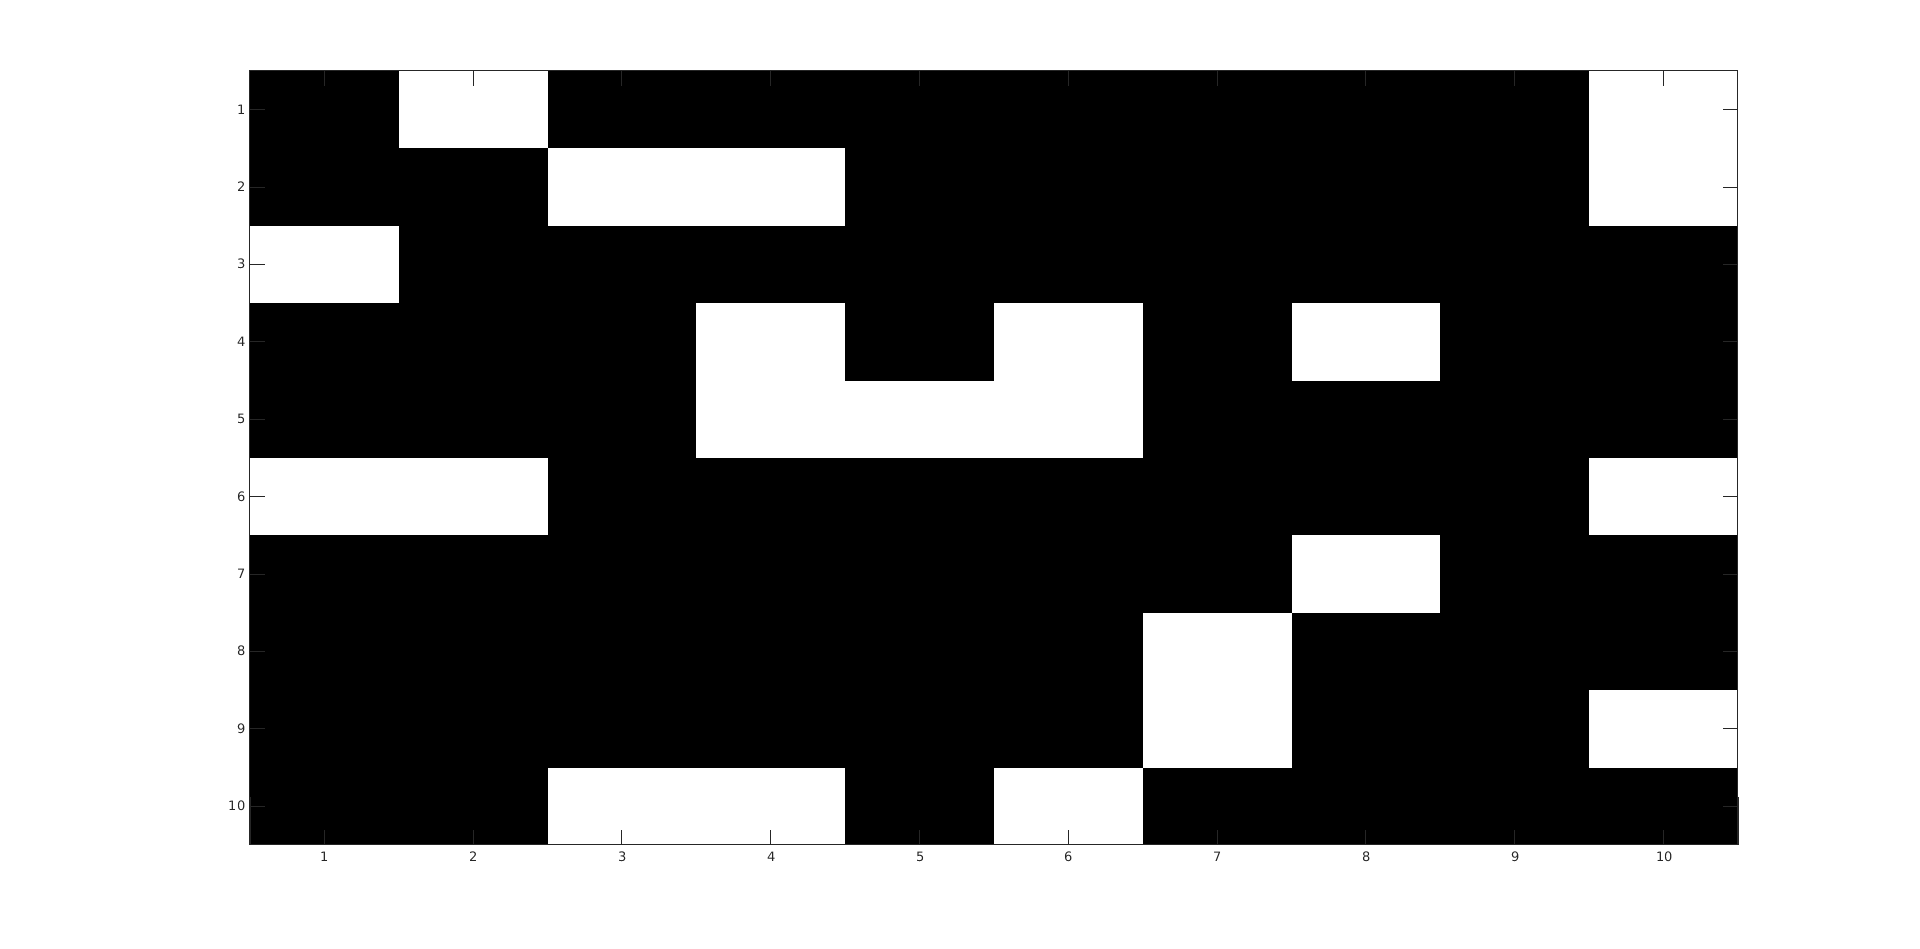
\includegraphics[width = 140mm]{../Figures/porousMedium10x10.png}
  \caption{Porøst medium for $L=10$}
  \label{fig:fig7}
  \end{center}
\end{figure}

\noindent
Perkolasjon er studiet av konduktivitet i porøse medier. Det vi vil finne ut av er om det finnes en sammenhengende
sti fra den ene siden av materialet til den andre? Dette avhenger av $p$. $p_c$, perkolasjonsterskelen, er den 
verdien av $p$ som gjør at vi først får en sti som spenner over hele materialet. $p_c$ vil ha forskjellige verdier
for forskjellige realiseringer av matrisen over, derfor må vi se på $p_c$ enten som et statistisk gj.snitt 
eller se på den termodynamiske grensen, dvs. for et uendelig stort system. Det sistnevnte er det vi gjør. 
$p_c$ avhenger av rule-of-connectivity, dvs. om vi definerer connectivitiy som nearest-nabo eller
next-nearest-nabo, dvs. $Z=4$ og $Z=8$ respektivt, og av formen på sitesene. Man kan derimot utlede
mange ting som ikke avhenger av dette, men som er universelle. Dersom vi antar at de okkuperte sites
er hull, vil porøsiteten bli $\Phi = p$. \\

\noindent
For å finne clusters, dvs. sites som er nearest-neighbours, gjør vi slik:
\begin{lstlisting}
 [lw,num] = bwlabel(m,4);
\end{lstlisting}
Funksjonen \textit{bwlabel} returnere matrisen $lw$ som for hver site i $m$ angir med en indeks hvilken 
cluster denne siten tilhører. Clusterne gis indekser i stigende rekkefølge. Vi visualiserer
ved å gi hver cluster hver sin farge:
\begin{lstlisting}
 img = label2rgb(lw, 'jet', 'k', 'shuffle');
 image(img);
\end{lstlisting}
som ser slik ut
\begin{figure}[H]
  \begin{center}
  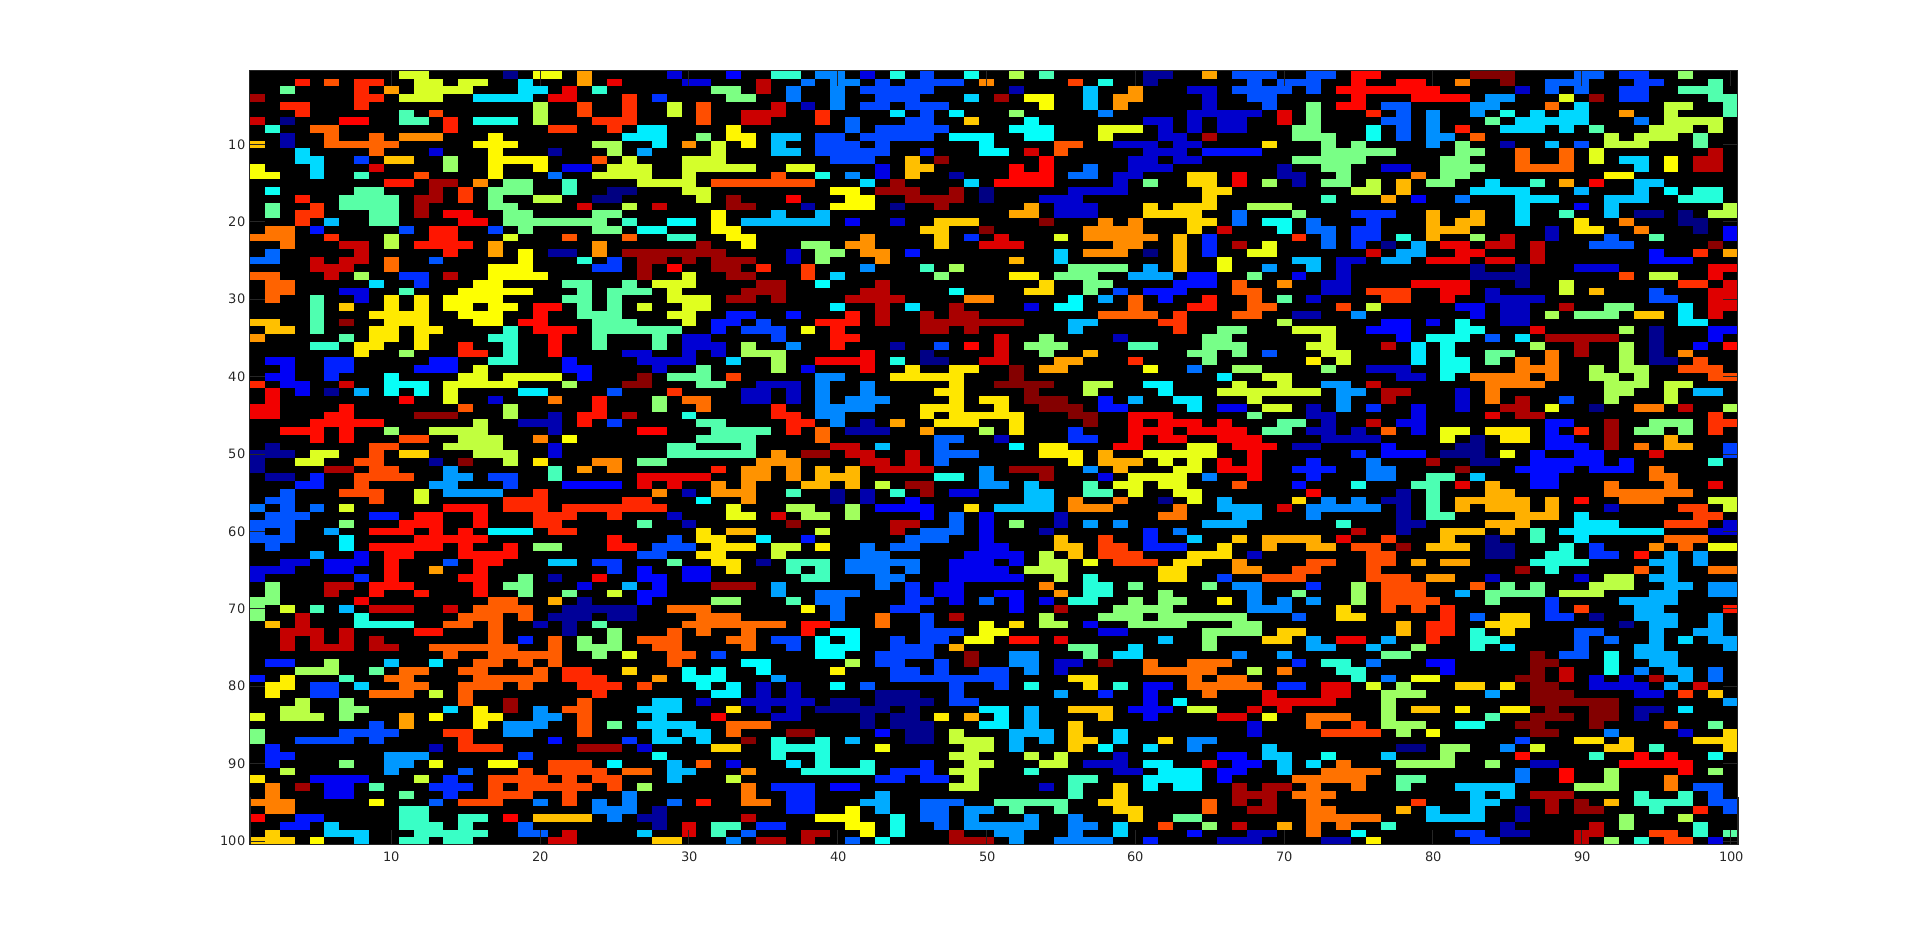
\includegraphics[width = 140mm]{../Figures/clusters100x100.png}
  \caption{Clusters for $L=100$ og $p=0.4$}
  \label{fig:fig7}
  \end{center}
\end{figure}

\subsubsection{Percolation probability}
Perkolasjonssannsynlighetet $\Pi(p,L)$ er definert som sannsynligheten for at det er en 
sammenhengende sti fra den ene siden til den andre som funksjon av $p$ i et system av størrelse $L$. 
Vi kan måle $\Pi(p,L)$ ved å lage $N$ random matriser for hver verdi av $p$, og telle hvor mange ganger vi 
har en spanning cluster for hver $p$. Til slutt deler vi på antall samples $N$:
\begin{lstlisting}
p = (0.4:0.01:1.0);
nx = length(p);
Ni = zeros(nx,1);
N = 10;
L = 100
for i = 1:N
    % generate new realization for each Ni
    z = rand(L,L);
    for ip = 1:nx
        m = z < p(ip);
        % finds clusters
        [lw,num] = bwlabel(m,4);
        % find spanning clusters
        top = lw(1,:);
        bottom = lw(L(j),:);
        left = lw(:,1);
        right = lw(:,L(j));
        % check whether the same cluster is at opposite ends of grid
        % intersect finds indicies that are the same in the two arrays,
        % without repetition
        tb = intersect(top,bottom);
        lf = intersect(left,right);
        % don't want to count the same cluster twice
        % union combines the data in tb and lf with no repetitions
        sc = union(tb,lf);
        % remove the unoccupied cluster
        sc = sc(sc~=0);
        if ~isempty(sc);
            Ni(ip) = Ni(ip) + 1
        end
    end
end
Pi = Ni/N;
plot(p,Pi);
\end{lstlisting}


\subsection{11 15 Percolation on small lattices}
\textit{Discuss the percolation problem on a 2x2 lattice. Sketch $P(p,L)$ and $\Pi(p,L)$ for small L.
Relate to your simulations. How to find spanning clusters and measure the percolation probability?} \\

\subsubsection{Density of spanning cluster}
Tettheten $P(p,L)$ til en spanning cluster er definert som sannsynligheten for at en random site
tilhører en spanning cluster:
\begin{equation}
 P(p,L) = \frac{M_s}{L^2}
\end{equation}
der $M_s$ er massen til clusteren, dvs. hvor mange sites den inneholder. Denne måles ved samme
metode som for $\Pi(p,L)$, bare at nå trenger vi en måte å finne massen til spanning cluster på. 
Dette gjøres slik:
\begin{lstlisting}
 s = regionprops(lw, 'Area')
 area = cat(1,s.Area)
\end{lstlisting}
Hvis vi definerer massen til spannning cluster som massen til alle clusterne som spanner (dersom det 
er flere enn én), vil programmet se ut som det ovenfor, med en liten modifikasjon, slik at 
vi slipper å bruke regionprops-funksjonen. 
\begin{lstlisting}
p = (0.4:0.01:1.0);
nx = length(p);
Mi = zeros(nx,1);
N = 10;
Lx = 500;
Ly = 20;
for i = 1:N
    % generate new realization for each Ni
    z = rand(Lx,Ly);
    for ip = 1:nx
        m = z < p(ip);
        % finds clusters
        [lw,num] = bwlabel(m,4);
        % find spanning clusters
        top = lw(1,:);
        bottom = lw(L(j),:);
        left = lw(:,1);
        right = lw(:,L(j));
        tb = intersect(top,bottom);
        lf = intersect(left,right);
        sc = union(tb,lf);
        if ~isempty(sc);
            for j = 1:length(sc)
                Mi(j) = Mi(j) + length(find(lw == sc(k)));
            end
        end
    end
end
P = Mi/N;
plot(p,Pi);
\end{lstlisting}
\begin{figure}[H]
  \begin{center}
  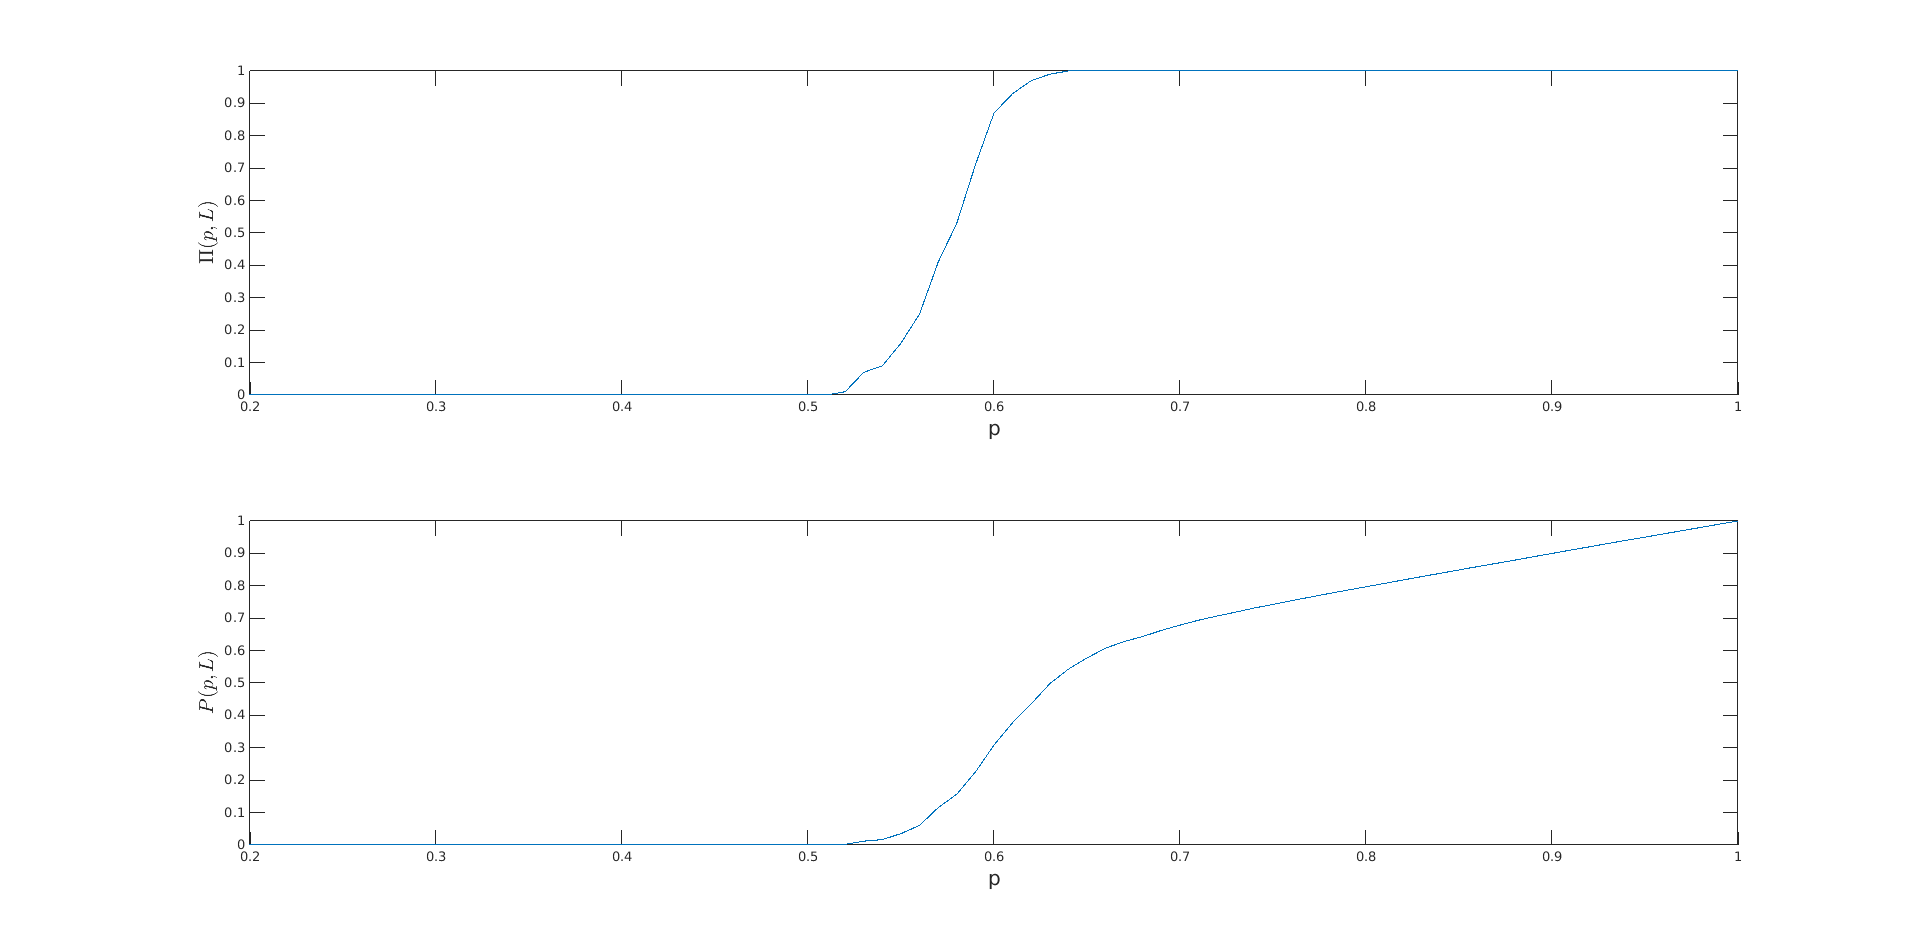
\includegraphics[width = 140mm]{../Figures/PiAndPL50.png}
  \caption{Percolation probability and density of spanning cluster for $L=50$}
  \label{fig:fig7}
  \end{center}
\end{figure}
Vi ser at $\Pi$ har rask økning noe før $p_c = 0.59275$ opp til 1. $\Pi$ går mot en stepfunksjon
når $L$ går mot uendelig. $P$ har samme oppførsel før $p_c$, men etter øker den lineært med $p$, dette
fordi når $p$ er nære 1 vil nesten alle okkuperte sites være del av spanning cluster. Når vi øker $p$
vil det komme flere okkuperte sites, som også vil være del av spanning cluster, derfor lineær økning i $p$. 

\subsubsection{Percolation on 2x2 lattice}
Kurvene ovenfor vil bli mer og mer linære for mindre $L$. For $L=1$ har vi $\Pi(p,1) = p$ og $P(p,1) = p$,
dersom den ene siten er okkupert, har vi perkolasjon, hvis ikke, har vi ikke perkolasjon. 
Vi kan også finne eksakte resultater for $L=2$. Da må vi liste opp alle mulige konfigurasjoner,
det er totalt $2^4 = 16$ muligheter (generelt: $2^{L^2}$), og finne sannsynligheten til hver konfigurasjon. 
I tillegg bruker vi fra sannsynlighetsteori at
\begin{equation}
 P(A) = \sum_B P(A|B)P(B)
\end{equation}
som vil si at sannsynligheten for $A$ er gitt som sannsynligheten for $A$ gitt $B$ ganget med
sannsynligheten for $B$, summert over alle mulige utfall for $B$. Vi kan dermed finne
Perkolasjonssannsynligheten ved
\begin{equation}
 \Pi(p,L) = \sum_c \Pi(p,L|c)P(c)
\end{equation}
der vi summer over alle mulige konfigurasjoner $c$. Det vil generelt bli et polynom av grad $L^2$, men denne
teknikken er ikke realistisk i lengden fordi mulige utfall blir veldig stort. Sannsynligheten for
konfigurasjonene der en site er fylt, er like, nemlig $p(1-p)^3$. Alle disse bidrar null til $\Pi$ fordi
perkolasjon er umulig når kun en site er okkupert. 
Slik ser det ut for $L = 1,2,3,4$:
\begin{figure}[H]
  \begin{center}
  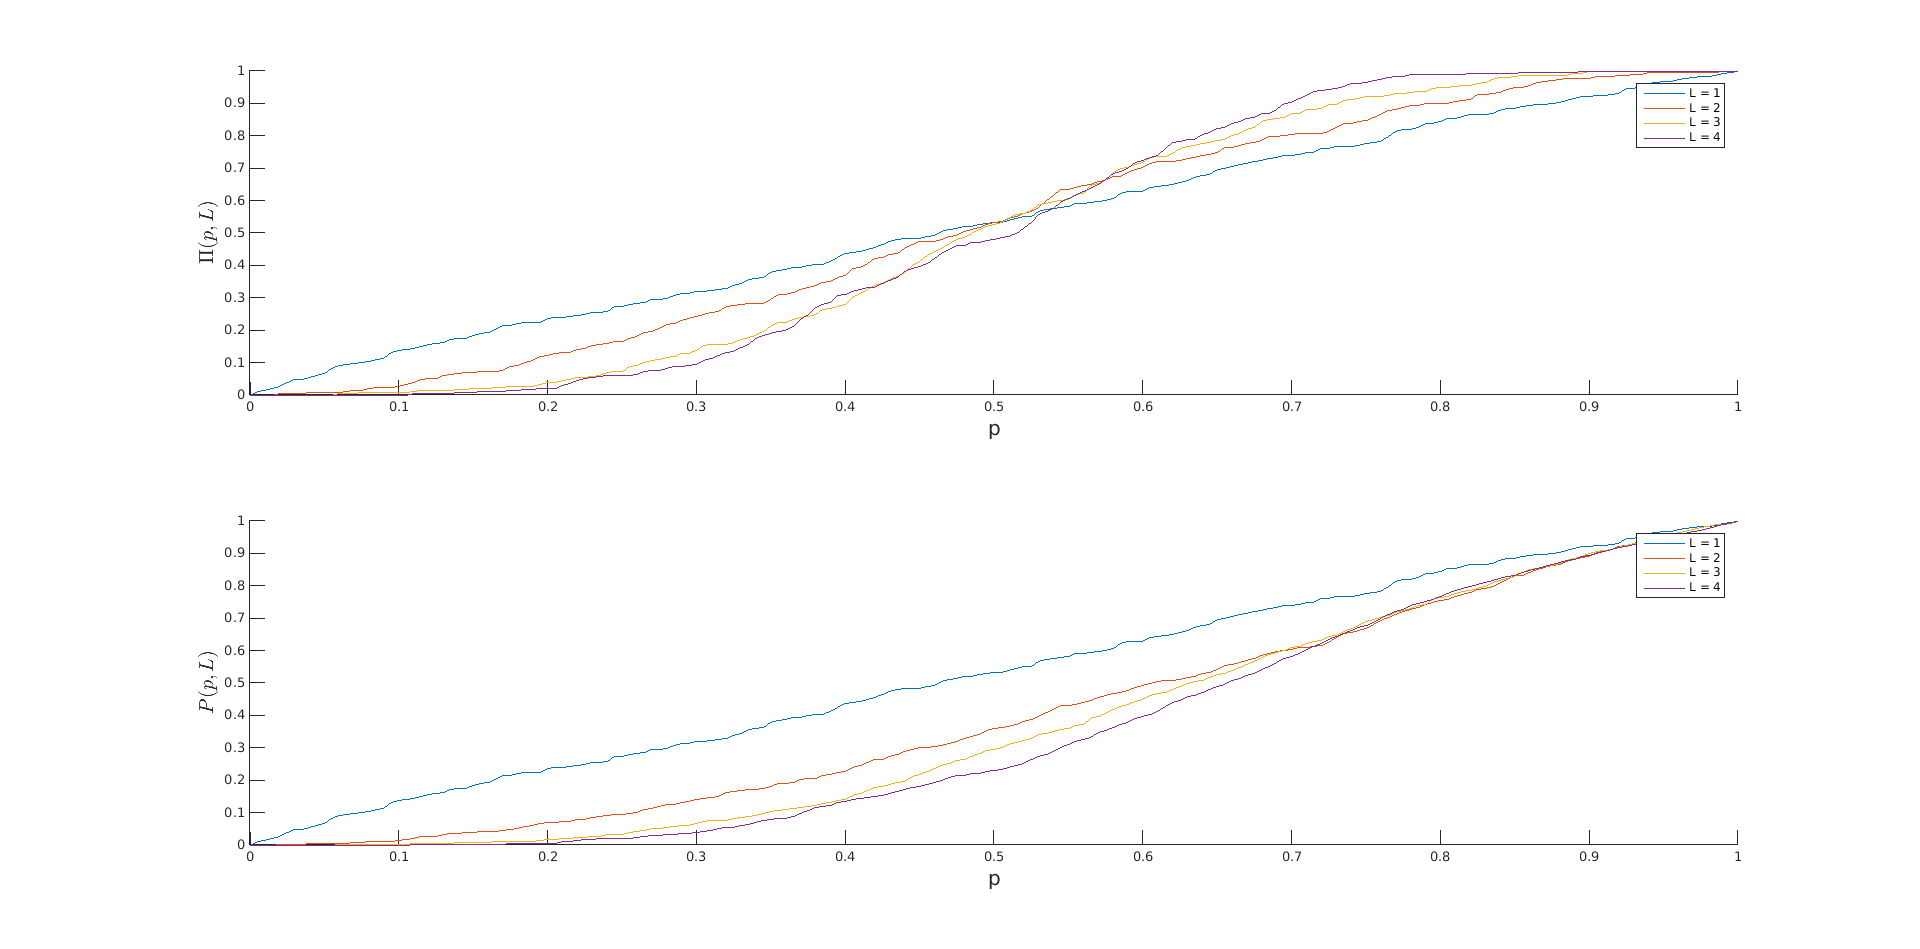
\includegraphics[width = 140mm]{../Figures/PiAndPL1234.png}
  \caption{Percolation probability and density of spanning cluster for $L=1,2,3,4$}
  \label{fig:fig8}
  \end{center}
\end{figure}
For $P$ får vi følgende verdier:
\begin{table}[H] 
  \begin{center}
    \begin{tabular*}{8cm}{@{\extracolsep{\fill}} cccc}
      \toprule
      $c$ & $g_c$ & $\hat{P}(c)$ & $P(p,2|c)$ \\ 
      \hline
      1 & 1 & $p^0(1-p)^4$ & 0 \\
      2 & 4 & $p^1(1-p)^3$ & 0 \\ 
      3 & 4 & $p^2(1-p)^2$ & 1/2 \\ 
      4 & 2 & $p^2(1-p)^2$ & 0 \\ 
      5 & 4 & $p^3(1-p)^1$ & 3/4 \\
      6 & 1 & $p^4(1-p)^0$ & 1 \\
      \bottomrule
      \end{tabular*} 
    \end{center}
      \caption {Probabilites for the different configurastions $c$. $\hat{P}(c)$ er sannsynligheten
                for konfigurasjon $c$, $P(p,2|c)$ er sannsynligheten for at en site er del av en 
                spanning cluster gitt konfigurasjon $c$.}
  \label{tab:HOEnergies} 
\end{table}
Vi får dermed
\begin{equation}
 P(p,2) = 2p^2(1-p)^2 + 3p^3(1-p) + p^4
\end{equation}

\subsection{12 14 16 Cluster number density in 1d percolation}
\textit{Define the cluster number density for 1d percolation, and show that it can be measured. 
Discuss the behaviour when $p \to p_c$. How does it relate to your simulations in two-dimensional 
systems?} \\
\textit{Introduce the characteristic cluster size for the 1-d percolation problem, and discuss their
behaviour when $p \to p_c$. Relate to your simulations on two-dimensional percolation}\\
\textit{Introduce the cluster number density and its applications: Definition, measurement, scaling
and data-collapse. }\\

\noindent
Cluster number density er definert som sannsyniligheten for at en random site er en spesifikk site
i en cluster av størrelse $s$. For 1d har vi
\begin{equation}
 n(s,p) = (1-p)^2 p^s
\end{equation}
som betyr at vi må ha $s$ fylte sites med to tomme sites på hver side. $sn(s,p)$ er derfor sannsynligheten
for at en random site tilhører en cluster av størrelse $s$. Vi kan tenke på $n(s,p)$ som antalltettheten
til en cluster av størrelse $s$, dvs.
\begin{equation}
 \overline{sn(s,p)} = \frac{sN_s}{L^d}
\end{equation}
der $N_s$ er antall clusters av størrelse $s$, dvs. at $n(s,p)$ angir hvor mange sites som tilhører
clusters av størrelse $s$ i forhold til totalt antall sites, altså er $n(s,p)$ cluster-størrelse-
distribusjonen. 
$n(s,p)$ kan derfor måles slik:
\begin{equation}
 \overline{n(s,p)} = \frac{N_s}{L^d}
\end{equation}
For å få et statistisk godt resultat (størrelsen ovenfor vil variere for hver realisering)
må vi måle $N_s$ mange ganger, mange samples:
\begin{equation}
 \overline{n(s,p)} = \frac{N_s(M)}{ML^d}
 \label{measureNsp}
\end{equation}
der $M$ er antall samples eller realiseringer av systemet. 
Vi forventer at denne verdien ikke er eksakt fordi vi har et endelig antall samples og systemstørrelse $L$.
Den målte verdien vil gå mot den eksakte når $M$ og $L$ går mot uendelig. \\

\noindent
Denne distribusjonen er normalisert:
\begin{equation}
 p = \sum_{s=0}^\infty sn(s,p) + P
\end{equation}
dvs. at en okkupert site (sannsynlighet $p$) enten er en del av en endelig cluster av størrelse $s$, eller
del av den uendelige clusteren, som har sannsynlighet $P$. \\

\subsubsection{Characteristic cluster size}
For å se på den direkte $s$-avhengigheten for forskjellige $p$ kan vi plotte
\begin{equation}
 (1-p)^{-2}n(s,p) = p^s
\end{equation}
mot $s$ for forskjellige p, som vil se slik ut:
\begin{figure}[H]
  \begin{center}
  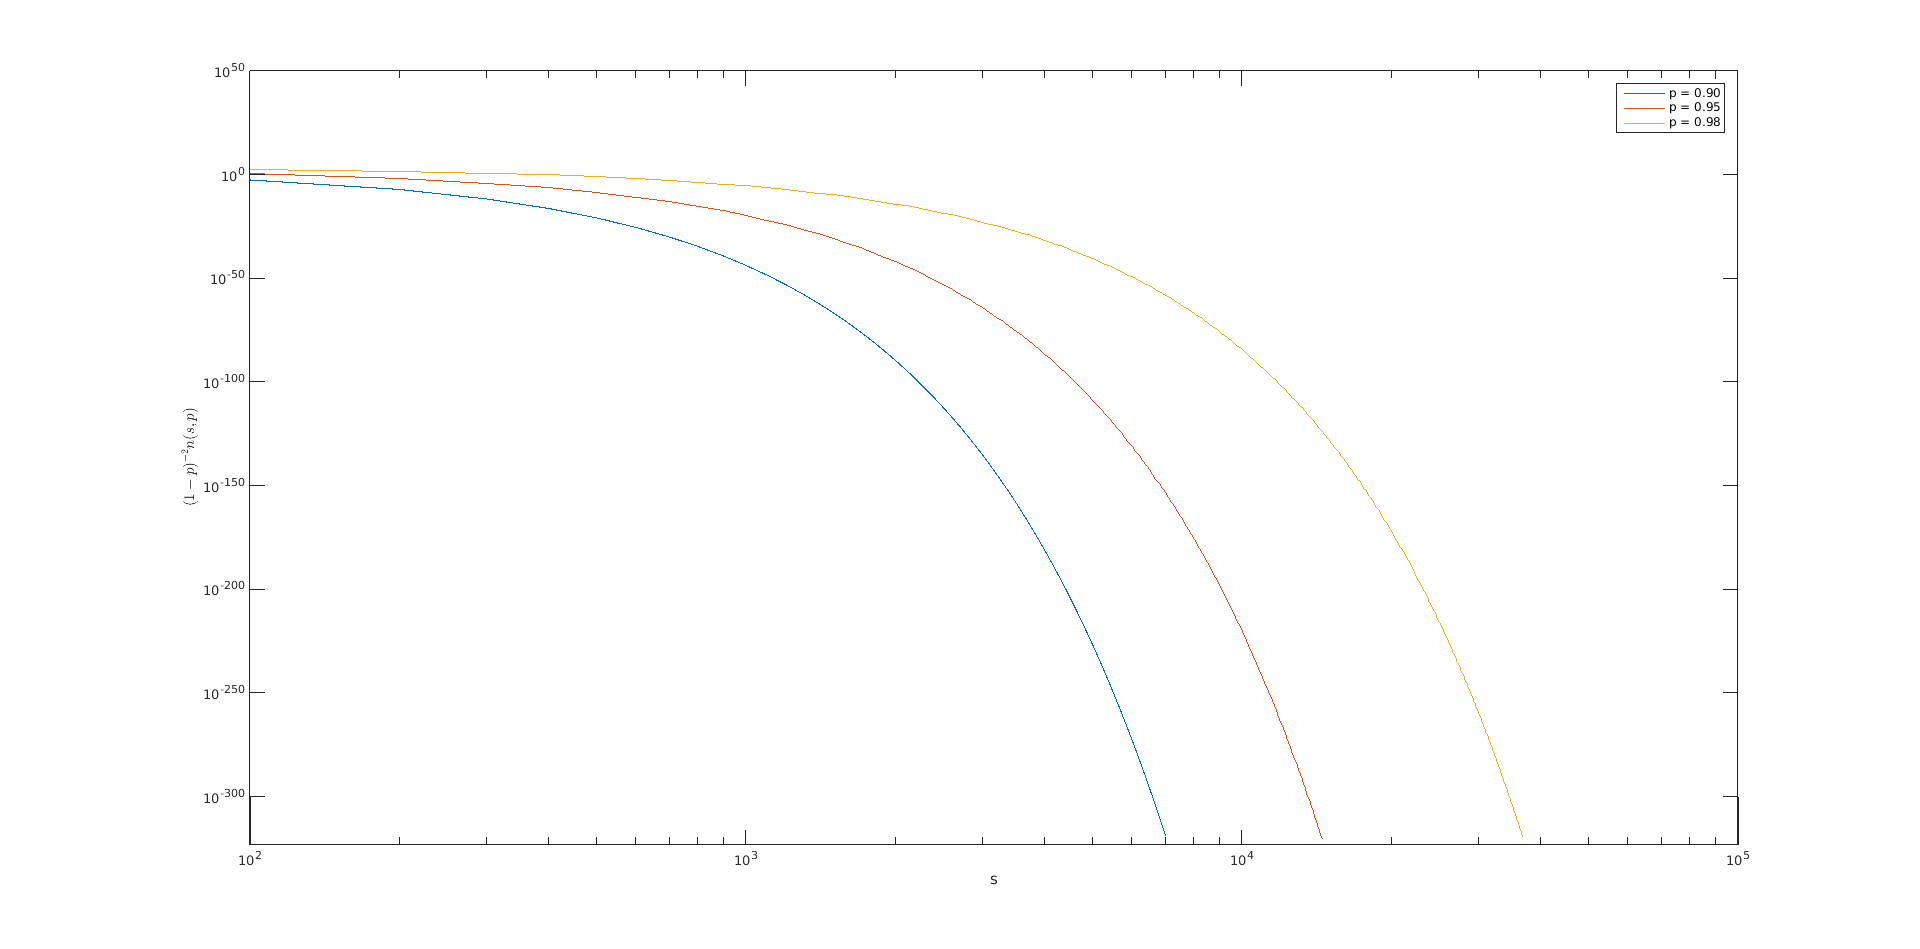
\includegraphics[width = 140mm]{../Figures/cnd1d.png}
  \caption{Cluster number density for increasing $p$}
  \label{fig:fig8}
  \end{center}
\end{figure}
For 1d har vi at $p_c = 1$. Vi ser at for alle $p$ er kurven noenlunde konstant for små $s$, før den faller
bratt. Vi kan definere en cut-off-størrelse $s_\xi$, denne øker når $p\to 1$ som vi ser fra plottet.
Vi kan skrive $n(s,p)$ som
\begin{equation}
 n(s,p) = (1-p)^2e^{s\ln{p}} = (1-p)^2e^{-s/s_\xi}
\end{equation}
hvor cut-off størrelsen er 
\begin{equation}
 s_\xi = -\frac{1}{\ln{p}}
\end{equation}
Når $p \to p_c = 1$ vil $s_\xi$ divergere. I denne grensen har vi at $1-p \ll 1$ og vi kan skrive
\begin{equation}
 \ln{p} = \ln{[1 - (1-p)]} \approx -(1-p)
\end{equation}
hvor vi har brukt Taylor-ekspansjonen $\ln{(1-x)} = -x + O(x^2)$ rundt $x=0$. Vi får dermed
\begin{equation}
 s_\xi \approx \frac{1}{1-p} = \frac{1}{p_c - p} = |p-p_c|^{-1/\sigma}
\end{equation}
hvor $\sigma$ er en universell eksponent, dvs. at den ikke avhenger av lattice-detaljer. 
\begin{equation}
 s_\xi \propto |p - p_c|^{-1/\sigma}
\end{equation}
Dette gjelder generelt for perkolasjonsteori, vi har altså denne oppførselen også i to dimensjoner. 
Vi kan her generere en datakollaps, dvs. at vi kan finne en skaleringsfunksjon ved det kritiske punktet
$p \to p_c$ som ikke avhenger av $L$ eller $p$, dermed bør alle kurvene i plottet ovenfor falle sammen.
Disse skaleringsfunksjonen vil alltid være potensfunksjoner av dimensjonsløse størrelser. 
Dette oppnår vi ved å plotte som en funksjon av $s/s_\xi$:
\begin{figure}[H]
  \begin{center}
  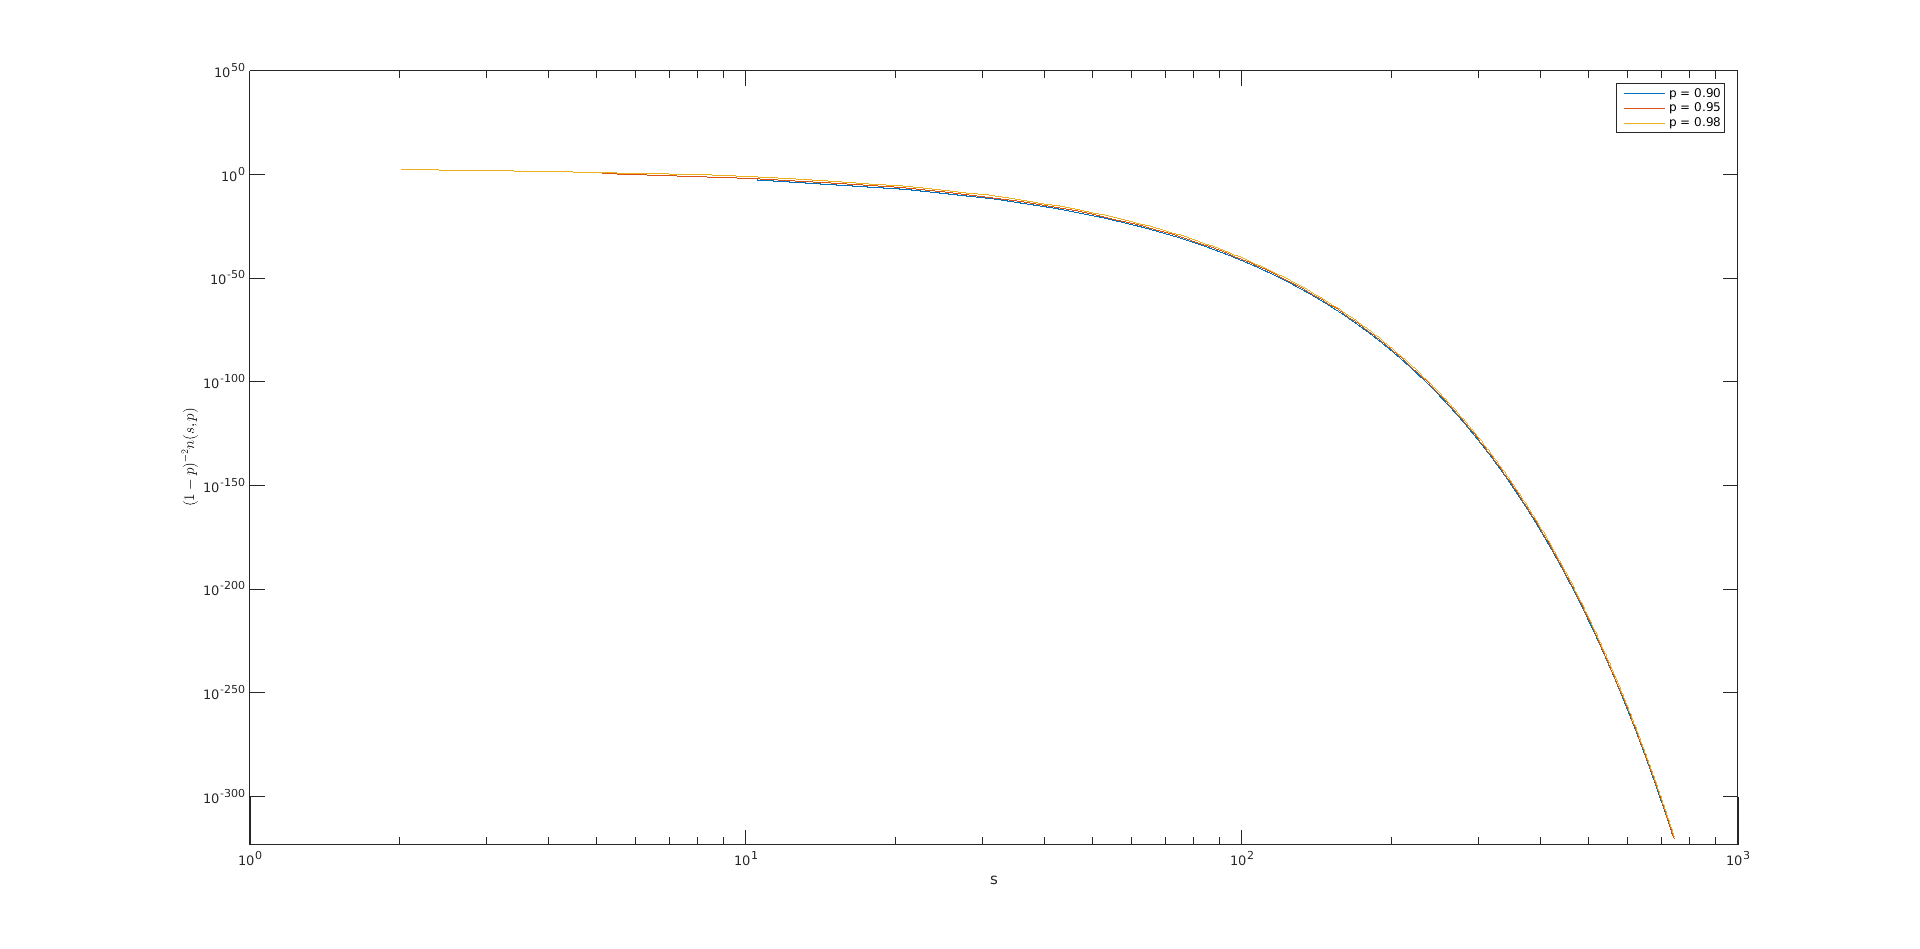
\includegraphics[width = 140mm]{../Figures/cndDataCollapse1d.png}
  \caption{Cluster number density for increasing $p$}
  \label{fig:fig9}
  \end{center}
\end{figure}
Siden $s_\xi \approx (1-p)^{-1}$ har vi at $(1-p)^2 = s_\xi^{-2}$ som gir
\begin{equation}
 n(s,p) = s_\xi^{-2} e^{-s/s_\xi} = s^{-2}(s/s_\xi)^2e^{-s/s_\xi} = s^{-2}F(s/s_\xi)
\end{equation}
der $F(u) = u^2e^{-u}$ er skaleringsfunksjonen. Dette gjelder også for alle dimensjoner:
\begin{equation}
 n(s,p) = s^{-\tau}F(s/s_\xi)
\end{equation}
bare med andre verdier for $\tau$, som også er en universell eksponent. Denne formen ser vi
fra simulasjoner i 2d. 

\subsubsection{Numerical measurement}
Vi måler $n(s,p)$ på noenlunde samme måte som for $P(p,L)$. Vi bruker area-funksjonen for å 
finne massen til alle clusters for ulike $p$, etter vi har fjernet spanning cluster. Dette gjør vi 
$M$ ganger, for hver $M$ legger vi til area-vektoren til en total vektor:
\begin{lstlisting}
        % find and remove spanning cluster
        top = lw(1,:);
        bottom = lw(L,:);
        left = lw(:,1);
        right = lw(:,L);
        tb = intersect(top,bottom);
        lf = intersect(left,right);
        sc = union(tb,lf);
        % remove sites that are not part of clusters
        % sc now contains the indicies of eventual spanning clusters
        sc = sc(sc~=0);
        if ~isempty(sc);
            for k = 1:length(sc);
                % remove spanning clusters
                %length(sc)
                lw = lw(lw ~= sc(k));
            end
        end
        
        % find distribution of cluster sizes
        s = regionprops(lw, 'Area');
        % area contains number of sites in all clusters
        area = cat(1, s.Area);
        allarea = cat(1, allarea, area);
\end{lstlisting}
$allarea$ inneholder nå massen til alle clusterne målt $M$ ganger. Vi finner $N_s$ ved
å lage et histogram over denne vektoren:
\begin{lstlisting}
 [n,s] = hist(allarea, L^2)
\end{lstlisting}
der vi bruker $L^2$ bins slik at det blir en bin per cluster-størrelse $s$. $n$ angir hvor mange clusters
som er i hver bin, altså $N_s$. Til slutt finner vi $n(s,p)$ slik:
\begin{lstlisting}
 nsp = n/(L*M)
\end{lstlisting}
som i \eqref{measureNsp}. Vi måler $n(s,p$ på akkurat samme måte i 2d, bare at da bruker vi 
logaritmisk binning. Dvs. at binkantene er gitt som $a^i$ der $a$ er basis for binsene og
$i$ er binnummeret. Binene øker altså i størrelse med nummeret. Vi må da huske på å dele med 
binstørrelsen:
\begin{equation}
 \overline{n(s_i,p,L)} = \frac{N_i}{ML^d\Delta s_i}
\end{equation}

\subsubsection{Scaling and data collapse in 2d}
I 2d ser $n(s,p)$ slik ut når $p \to p_c$:
\begin{figure}[H]
  \begin{center}
  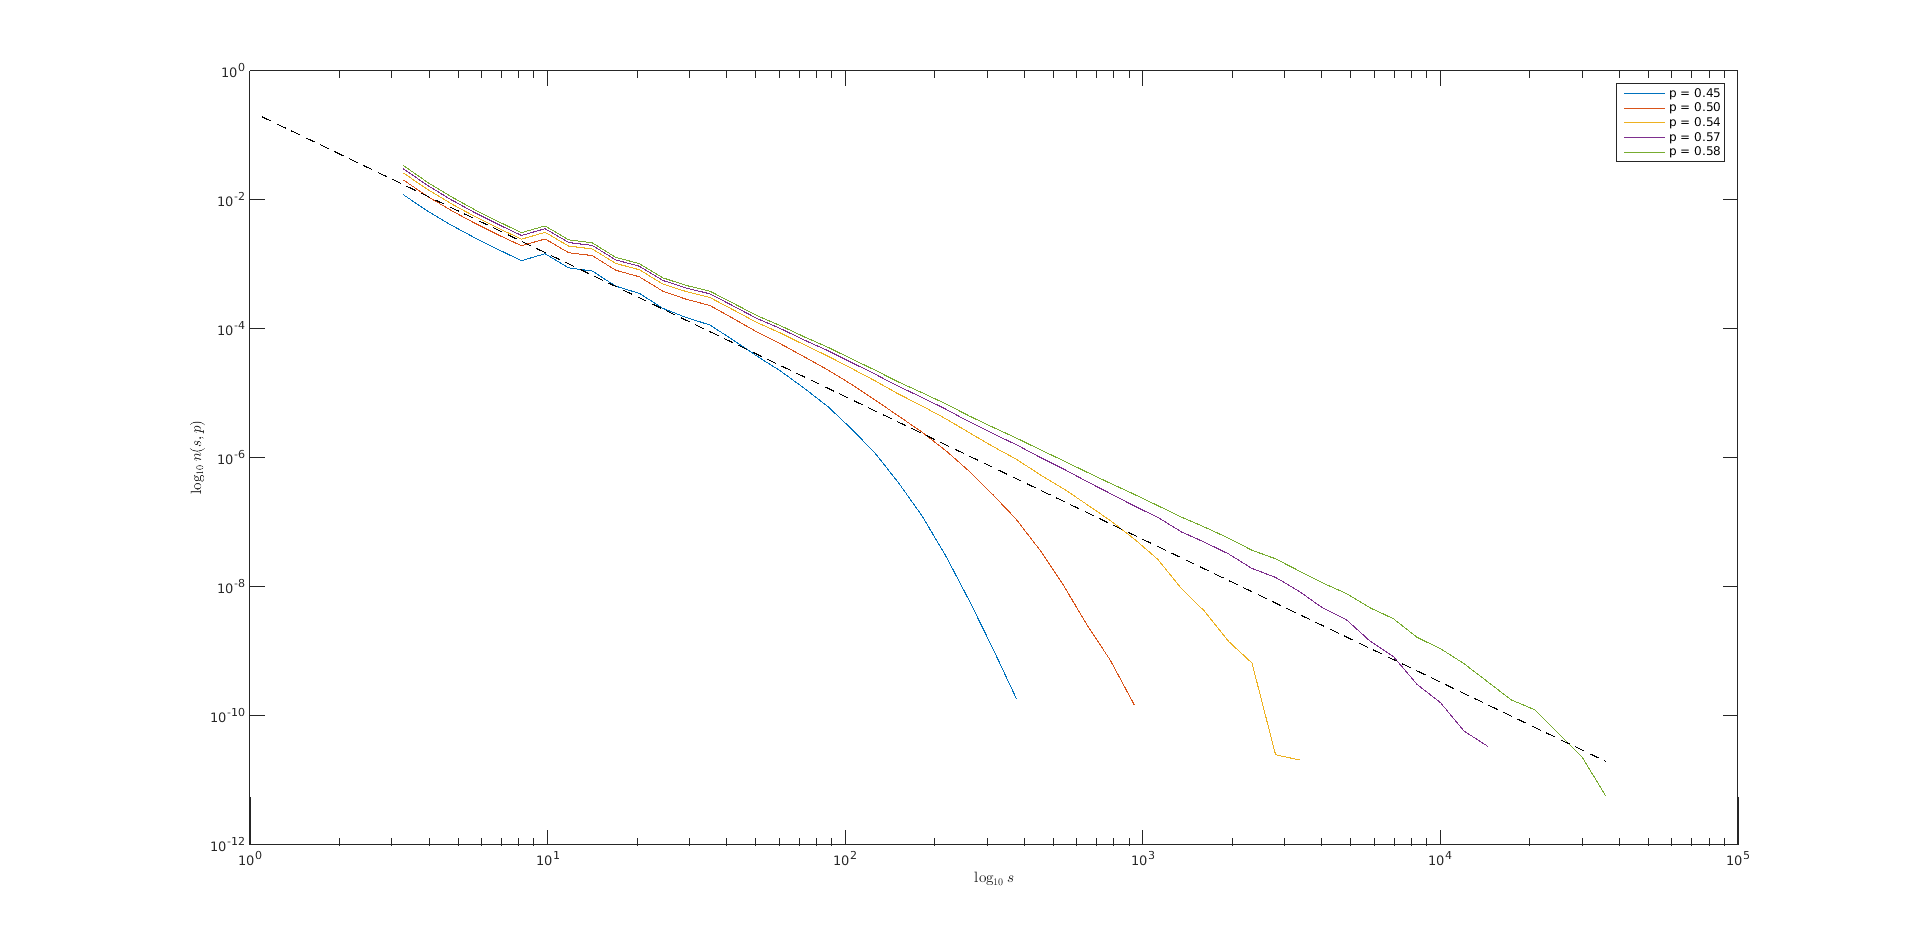
\includegraphics[width = 140mm]{../Figures/scalingClusterSize512.png}
  \caption{Cluster number density for increasing $p$}
  \label{fig:fig9}
  \end{center}
\end{figure}
\begin{figure}[H]
  \begin{center}
  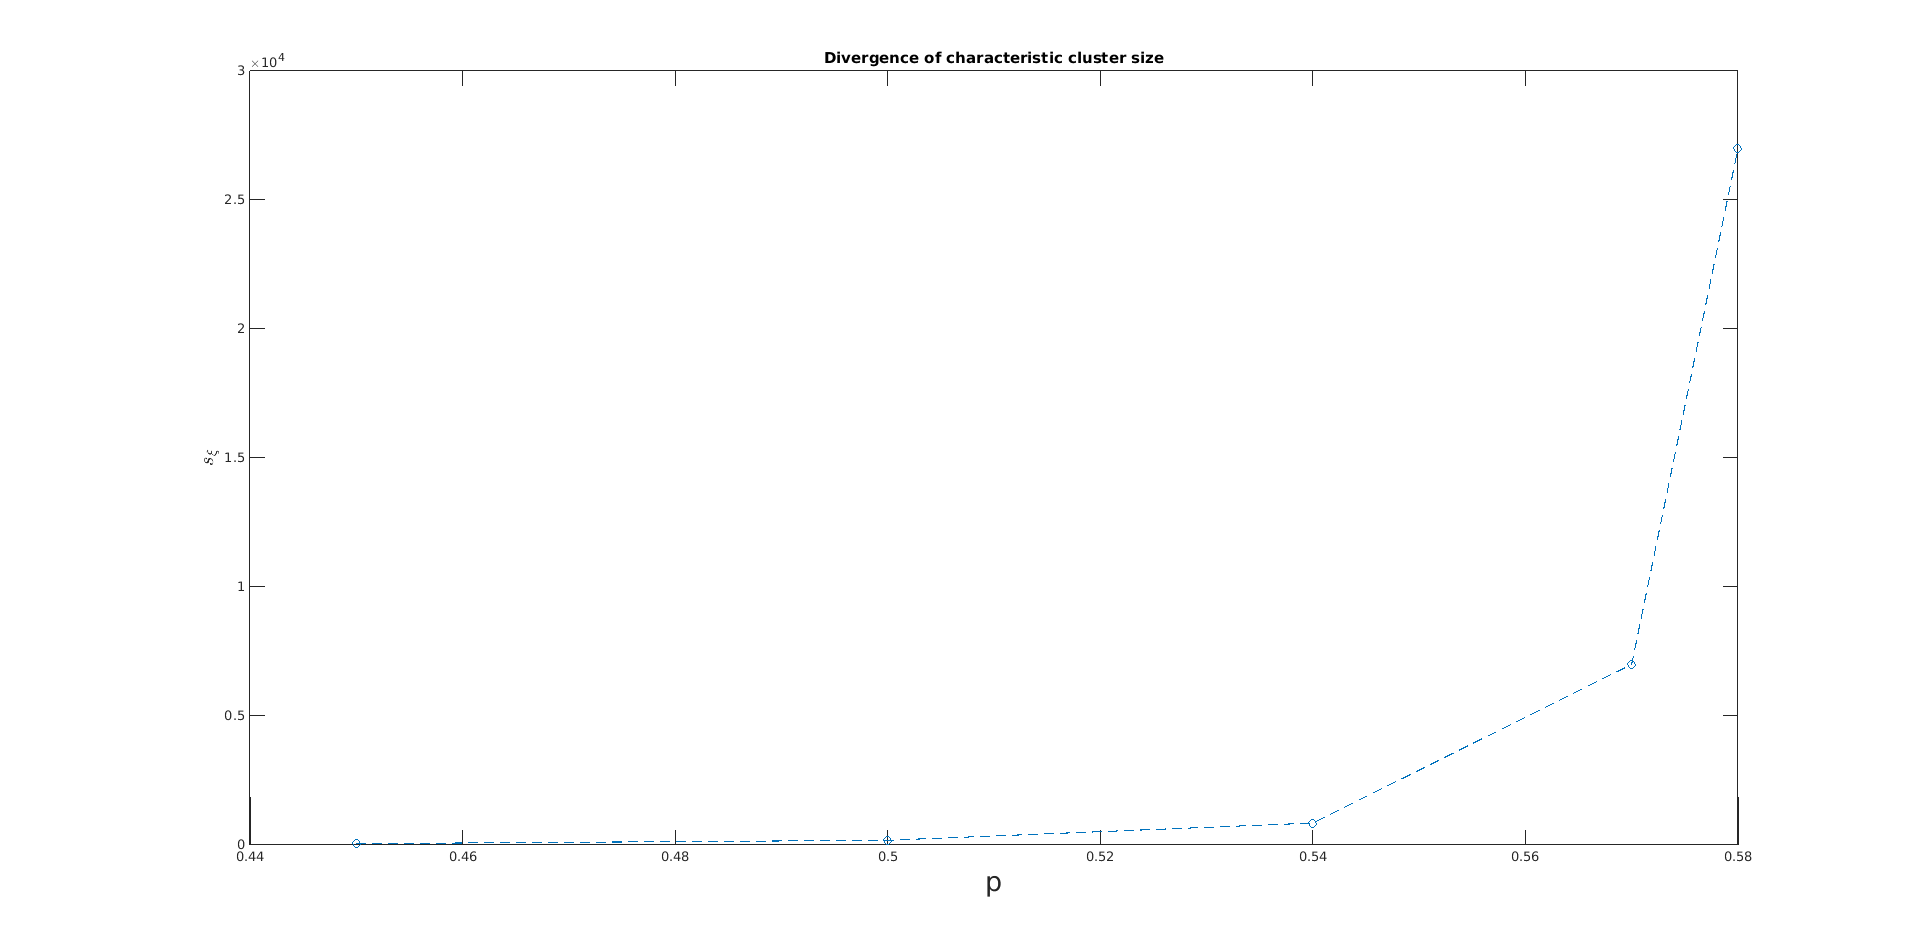
\includegraphics[width = 140mm]{../Figures/charClusterSizeDivergence.png}
  \caption{Divergence of $s_\xi \propto |p-p_c|^{-1/\sigma}$}
  \label{fig:fig10}
  \end{center}
\end{figure}
Vi ser at $n(s,p)$ har samme form i 1d som i 2d. $n(s,p) \propto s^{-\tau}$ for små $s$,
følger altså en potenslov, fram til $s_\xi$, der den faller bratt. Skjæringslinja
er senket med en faktor halv, og skjæringspunktene angir $s_\xi$ for økende $p$. Når vi så plotter
$s_\xi$ mot $p$, ser vi at $s_\xi \propto |p-p_c|^{-1/\sigma}$ som i 1d, og $\sigma$ kan regnes ut
ved å gjøre en 1d polynomisk fit. Vi har altså følgende skaleringsteori for $n(s,p)$:
\begin{equation}
 n(s,p) = n(s,p_c)F(s/s_\xi) \\
\end{equation}
\begin{equation}
 n(s,p_c) = Cs^{-\tau} \\
\end{equation}
\begin{equation}
 s_\xi = s_0|p-p_c|^{-1/\sigma}
\end{equation}
Vi kan finne $\tau$ ved å gjøre en lineær fit for $n(s,p_c,L)$ for økende $L$ før vi når $s_\xi$. 
$\sigma$ finner vi som beskrevet ovenfor vha. skjæringspunkter osv. Også her kan vi gjøre en datakollaps
for å finne skaleringsfunksjonen $F(s/s_\xi)$. Vi kan skrive
\begin{equation}
 n(s,p) = s^{-\tau}F(s(p-pc)^{1/\sigma})
\end{equation}
Hvis vi nå plotter $s^\tau n(s,p)$ mot $s(p-pc)^{1/\sigma}$, vil vi få en datakollaps fordi
vi da blir kvitt $p$-avhengigheten, skaleringsfunksjonen er uavhengig av $p$:
\begin{figure}[H]
  \begin{center}
  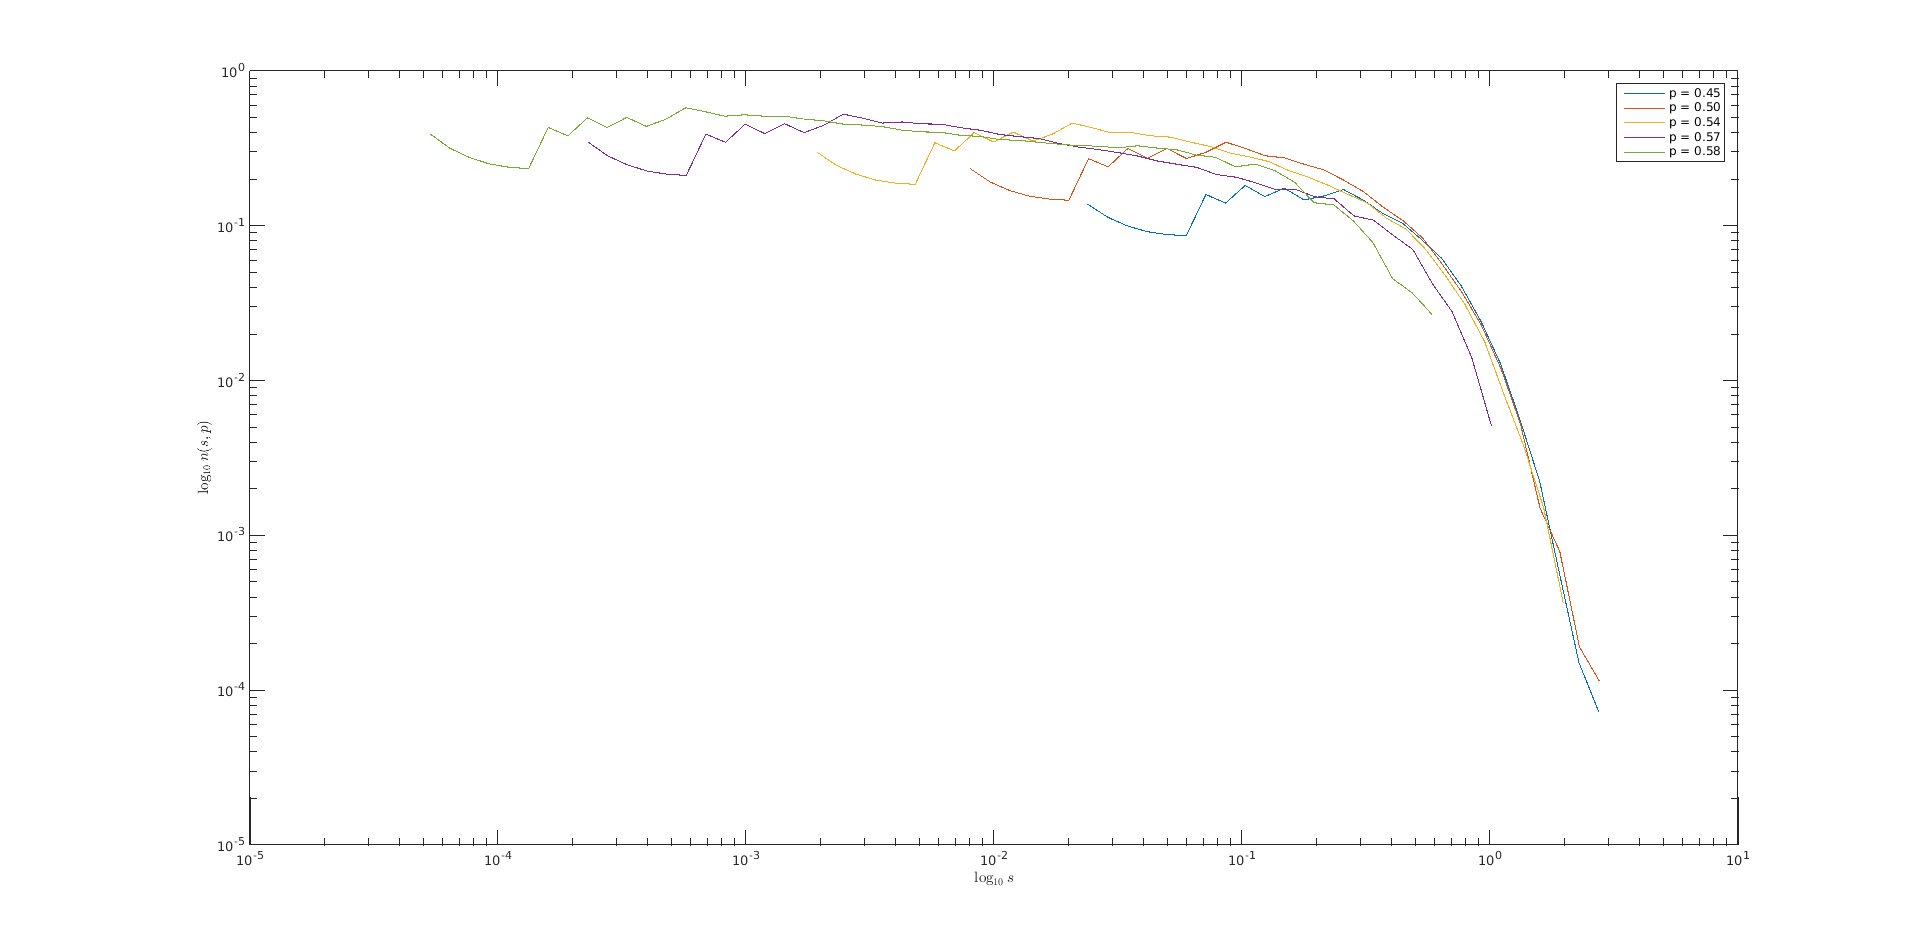
\includegraphics[width = 140mm]{../Figures/cndDataCollapse2d.png}
  \caption{Cluster number density for increasing $p$}
  \label{fig:fig9}
  \end{center}
\end{figure}
SKRIVE NOE OM AT VI KAN BRUKE N(S,P) TIL Å REGNE UT GJ.SN. CLUSTER-STØRRELSE?


\subsection{13 Correlation length in 1d percolation}
\textit{Define the correlation length $\xi$ for 1d percolation. Discuss its behaviour when
$p \to p_c$. How is it related to cluster geometry and your results for 2d percolation?}\\

\noindent
The characteristic cluster size $s_\xi$ sier noe om massen til en cluster. Vil vil også
gjerne si noe om størrelsen eller utstrekningen til en cluster. For karakterisere lineær
utstrekning av en kluster bruker vi korrelasjonsfunksjonen $g(r)$:
\indent \textit{$g(r)$ er sannsynligheten for at to sites $a$ og $b$, som begge er okkupert og
og separert ved en distanse $r$ tilhører samme cluster. }\\

\noindent
For 1d perkolasjon kan $a$ og $b$ bare være del av samme cluster dersom alle sites mellom er fylt. 
Dersom $r$ er antall sites mellom $a$ og $b$ (teller ikke med start- og sluttposisjon), så 
er korrelasjonsfunksjonen 
\begin{equation}
 g(r) = p^r = e^{r\ln{p}} = e^{-r/\xi}
\end{equation}
der $\xi = -1/\ln{p}$ er korrelasjonslengden, dvs. cut-off for $g(r)$. Vi har at
\begin{equation}
\ln{p} \simeq -(1-p)
\end{equation}
der vi har ekspandert $\ln{(1-x)}$ på samme måte som ovenfor. Vi har altså at
\begin{equation}
 \xi =  \frac{1}{1-p} = \frac{1}{p_c-p} = \xi_0|p - p_c|^{-\nu}
\end{equation}
med $\nu = 1$, som igjen er en universell eksponent som $\tau$ og $\sigma$, 
men $\nu$ avhenger av dimensjonen $d$. 
Vi ser at $\xi$ divergerer som en potenslov når $p \to p_c$, akkurat som $s_\xi$. 

\subsubsection{Finite system effects}
Så lenge $\xi \ll L$, vil vi ikke merke noe effekt av den endelige systemstørrelsen $L$ fordi
ingen clustere er store nok til å legge merke til den endelige størrelsen. Dersom $\xi \gg L$ derimot,
er oppførselen til systemet dominert av $L$, og det vil se ut som om vi har perkolasjon selv om 
vi muligens ikke har det, det blir umulig å avgjøre hvor nære vi er perkolasjon. Til nå har vi ikke 
tatt med at den øvre grensen for clusterstørrelse er $L$ og ikke $\infty$. 

\subsubsection{2d størrelse på clusters - radius of gyration}
I 2d bruker vi radius of gyration (rotasjonsradius) som et mål på størrelsen eller utstrekningen 
til en cluster. Rotasjonsradiusen er standardavviket i posisjon for en cluster. Rotasjonsradiusen
$R_i$ for en cluster $i$ av størrelse $s_i$ med sites ${\bf r}_j$ for $j = 1,\dots,s_i$ er definert som
\begin{equation}
 R_i^2 = \frac{1}{s_i}\sum_{j=1}^{s_i} ({\bf r}_j - {\bf r}_{cm,i})^2
\end{equation}
der ${\bf r}_{cm,i}$ er massesenteret til cluster $i$. En ekvivalent definisjon er
\begin{equation}
 R_i^2 = \frac{1}{2s_i}\sum_{n,m} ({\bf r}_n - {\bf r}_m)^2
\end{equation}
der summen går over alle sites $n$ og $m$ i cluster $i$, og vi må dele på antall ledd ganger 2 $2s_i^2$
fordi alle sites telles to ganger. For å finne en karakteristisk radius $R_s$ for en gitt cluster-størrelse $s$
midler vi over alle clusters med samme størrelse $s$
\begin{equation}
 R_s^2 = \langle R_i^2 \rangle_i
\end{equation}
For 1d er det bare en cluster for hver størrelse $s$, slik at $R_s^2 = R_i^2$:
\begin{equation}
 R_s^2 = \frac{1}{s} \sum_{i=1}^s(i - s/2)^2
\end{equation}
og vi får at 
\begin{equation}
 s \propto R_s
\end{equation}
i 1d. I 2d kan dette gjøres numerisk: Vi finner $R_i^2$ for alle clusters i en lattice $L\times L$, og deretter
midlet radius $R_s^2$ for alle $s$ med logaritmisk binning. Dette gjøres for flere $p$. Resultatet er
\begin{equation}
 s \propto R_s^D
\end{equation}
der $D = 1.89$ for 2d er dimensjonen til clusteren, fordi vi generelt har at masse (areal) og radius er
relatert $M \propto R^d$. En ikke-heltallsdimensjon viser at en cluster ved $p \to p_c$ er et fraktal. 
For hver verdi av $p$ har vi en karakteristisk masse $s_\xi$ og radius $R_{s_\xi}$ som er relatert
\begin{equation}
 s_\xi = R_{s_\xi}^D
\end{equation}
Vi har dermed følgende skalering
\begin{equation}
 R_{s_\xi} \propto (p - p_c)^{-1/\sigma D}
\end{equation}
der $\nu = 1/\sigma D$ er enda en universell eksponent. Vi kunne ha operert med gj.snittlige radius $R$
istedenfor en cut-off radius $R_{s_\xi}$, men etter mye utregninger kan vi vise at
\begin{equation}
 R \propto R_{s_\xi}
\end{equation}
vi trenger derfor bare operere med en av dem. $R_{s_\xi}$ er altså en cut-off-radius
for en cluster av størrelse $s$ for en gitt $p$ og $L$, mens $R$ er en gj.snittlig
radius for en cluster av størrelse $s$ for en gitt $p$ og $L$. Begge disse divergerer
når $p \to p_c$. 

\subsubsection{2d størrelse på clusters - korrelasjonslengde}
Vi kan også finne størrelsen av clusters ved korrelasjonslengden, som vi kan definere her
som gj.sn. kvadratisk avstand mellom to sites $i$ og $j$ som tilhører samme cluster. Korrelasjonsfunksjonen
$g(r)$ har den generell skaleringsformen
\begin{equation}
 g(r) = r^xf(r/\xi)
\end{equation}
der $x=0$ for 1d, som vi har sett ovenfor, og $f(r/\xi) = e^{-r/\xi}$. $f(u)$ går raskt mot null når
$u > 1$, mens for $u < 1$ er den cirka konstant. Etter mye utregninger kommer vi fram til at
\begin{equation}
 \xi \propto R \propto R_{s_\xi} \propto |p-p_c|^{-\nu} \propto s_\xi^{-D}
\end{equation}
$\xi$ er altså gj.sn. kvadrert avstand mellom to sites i en cluster, mens $R$-ene er gj.sn. standardavvik
i posisjoner for en cluster av størrelse $s$. Forøvrig har vi at
\begin{equation}
 M(p,L) \propto L^D
\end{equation}
fordi vi kan velge $L = \xi(p)$ for en gitt $p$. Dermed har vi at
\begin{equation}
 P(p,L) = \frac{M(p,L)}{L^d} \propto L^{D-d}
\end{equation}
og vi ser at tettheten avhenger av systemstørrelsen $L$, dvs. at clusteren er et fraktal. 
Vi har følgende skalering for $M$:
\begin{equation}
M(p,L) \propto
\begin{cases}
 L^D, & L \ll \xi \\
 \xi^{D-d} L^d & L \gg \xi
\end{cases}
\end{equation}


\subsection{ 17. Finite size scaling of $\Pi(p,L)$ }
\textit{Discuss the behaviour of $\Pi(p,L)$ in a system with a finite system size $L$. 
How can we use this to find the scaling exponent $\nu$ and the percolation treshold $p_c$?}\\

\noindent
I finite scaling sier noe om endring i et systems oppførsel når størrelsen er endelig. 
Vi deler inn i to kategorier:
\begin{enumerate}
 \item $L \ll \xi$, systemet ser ut som det er ved $p_c$, men vi kan ikke vite om det er det
 \item $L \gg \xi$, systemet er ca homogent ved lengder større enn $\xi$
\end{enumerate}
Vi vil studere den termodynamiske grensen ($L \to \infty$) til en størrelse $X(p)$ som
oppfører seg som en potenslov når $p \to p_c$, dvs. 
\begin{equation}
 X(p) \propto (p-p_c)^{-\gamma_x}
\end{equation}
Vi gjør følgende scaling ansats:
\begin{equation}
 X(p, L) = L^{\gamma_x/\nu} \chi(L/\xi)
\end{equation}
eller ekvivalent
\begin{equation}
 X(p,L) = L^{\gamma_x/\nu} \bar{\chi}(L/\xi)
\end{equation}
 
\subsubsection{For $\Pi(p,L)$}
Vi antar at $\Pi$ ikke har noen potensavhengighet av $\xi$, slik at
\begin{align}
 \Pi(p,L) &= \xi^0f(L/\xi) = f(L/\xi) \\
          &= f\left(\frac{1}{\xi_0(p-p_c)^{-\nu}}\right) \\
          &= f(\frac{L(p-p_c)^\nu}{\xi_0}) \\
          &= \hat{f}([L^{1/\nu}(p-p_c)]^\nu) \\
          &= \Phi[(p-p_c)L^{1/\nu}]
\end{align}
hvor vi har brukt at $\xi = (p-p_c)^{-\nu}$ og der $\hat{f}(u) = f(u/\xi_0)$ og
$\Phi(u) = \hat{f}(u^\nu)$. Vi kan bruke denne scaling ansatzen til å 
estimere $p_c$. Vi definerer
\begin{equation}
 p_{\Pi = x}(L)
\end{equation}
som den verdien av $p$ som gir $\Pi = x$, denne verdien er en funksjon av $p$. 
Setter inn dette i scaling ansatzen:
\begin{equation}
 x = \Phi[(p_{\Pi=x}(L) - p_c)L^{1/\nu}]
\end{equation}
som kan løses som 
\begin{equation}
 (p_{\Pi=x} - p_c)L^{1/\nu} = \Phi^{-1}(x) = C_x
\end{equation}
altså avhenger høyresiden kun av $x$ og ikke av $L$. Dette kan skrives
\begin{equation}
 p_{\Pi=x} - p_c = C_xL^{-1/\nu}
\end{equation}
Dersom vi har to $x$-verdier $x_1$ og $x_2$, får vi
\begin{equation}
 dp = p_{\Pi=x_1}(L) - p_{\Pi=x_2}(L) = (C_{x_1} - C_{x_2})L^{-1/\nu}
\end{equation}
altså kan vi plotte $\log(dp)$ som en funksjon av $\log(L)$ for å finne $\nu$, og så 
bruke likningen over til å finne $p_c$. Dette kan gjøres numerisk. Vi velger $x_1=0.3$ og $x_2=0.8$. 
For $L=[25,50,100,200,400,800]$ og for begge $x$ finner vi $\Pi(p,L)$, først for $p_c$. Dersom
vi får $\Pi(p,L) < x$ øker vi $p$, hvis ikke minker vi den. Denne algoritmen kjøres 10 ganger. Til 
slutt plotter vi $p_{\Pi = x}$ for begge $x$ som funksjon av $L$:
\begin{figure}[H]
  \begin{center}
  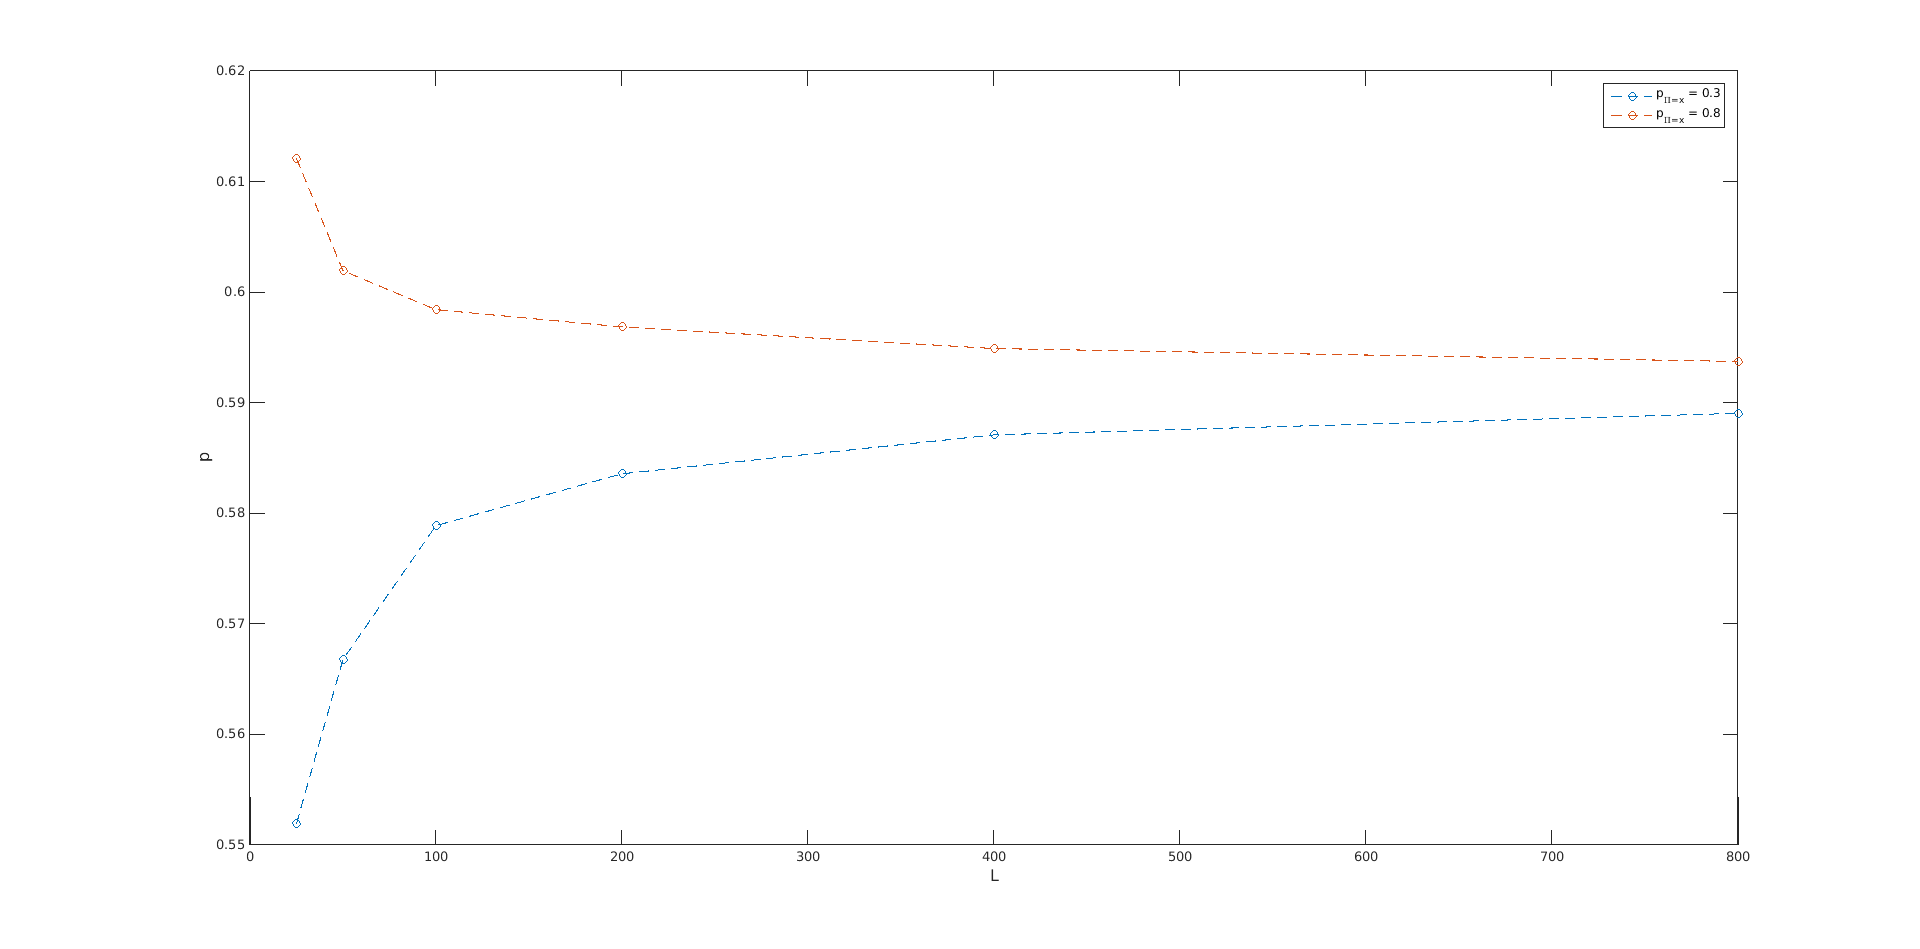
\includegraphics[width = 140mm]{../Figures/finiteScaling2.png}
  \caption{$p_{\Pi=x}$ for to $x$ som funksjon av systemstørrelse}
  \label{fig:fig10}
  \end{center}
\end{figure}
Vi ser at begge går $p\to p_c$ når $L$ øker, som forventet, $\Pi(p,L)$ går mot en stepfunksjon. For 
å finne $\nu$ plotter vi $p_{\Pi=0.3}(L) - p_{\Pi=0.8}(L)$ som funksjon av $L$ i loglog-plot:
\begin{figure}[H]
  \begin{center}
  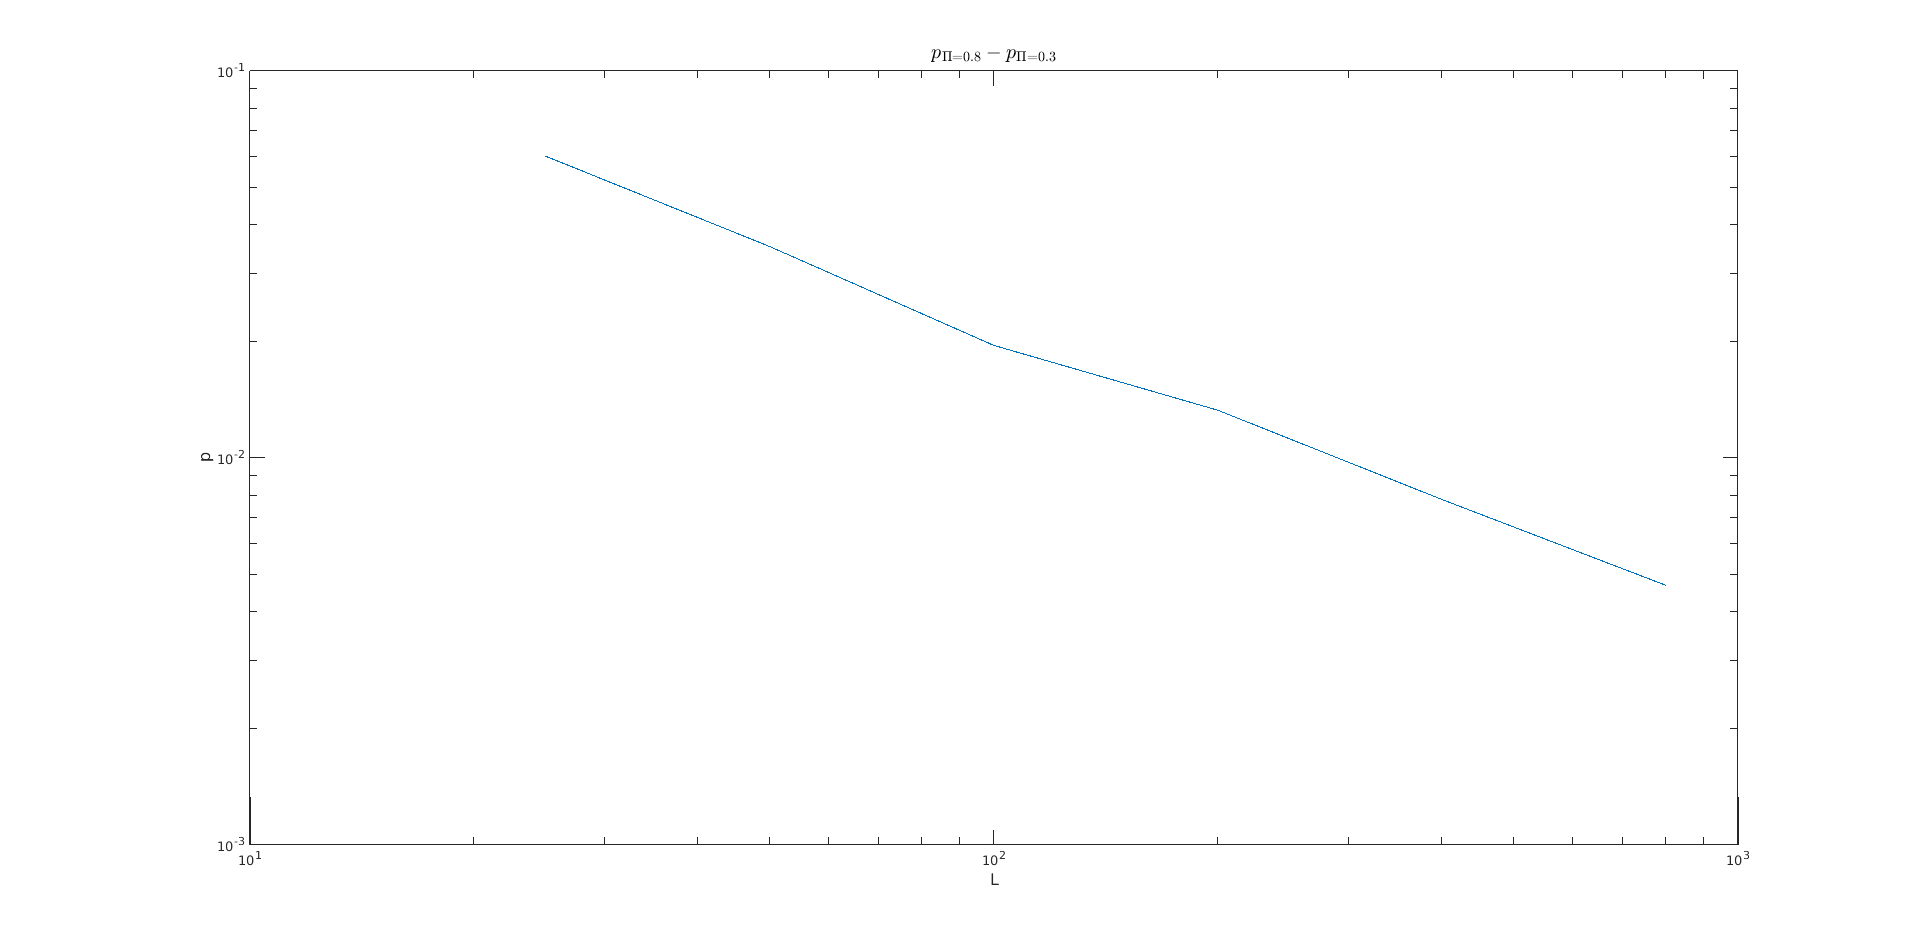
\includegraphics[width = 140mm]{../Figures/finiteScalingDp.png}
  \caption{Finner $\nu$}
  \label{fig:fig10}
  \end{center}
\end{figure}
Til slutt plotter vi $p_{\Pi=x}$ som funksjon av $L^{-1/\nu}$ for å estimere $p_c$, som vil være
skjæringspunktet med $y$-aksen. 
\begin{figure}[H]
  \begin{center}
  \includegraphics[width = 140mm]{../Figures/finiteScalingPiEsimatePc.png}
  \caption{$p_{\Pi=x}$ for to $x$ som funksjon av systemstørrelse}
  \label{fig:fig10}
  \end{center}
\end{figure}
Vi kan så plotte $\Pi(p,L)$ for flere $L$ som funksjon av $(p-p_c)L^{1/\nu}$ for å lage en datakollaps
for å finne skaleringsfunksjonen $\Phi$. Alle kurvene for forskjellige $L$ vil ligge oppå hverandre:
\begin{figure}[H]
  \begin{center}
  \includegraphics[width = 140mm]{../Figures/dataCollapsePi.png}
  \caption{Datakollaps for perkolasjonssannsynligheten}
  \label{fig:fig10}
  \end{center}
\end{figure}

\subsection{ 18. Subsets of the spanning cluster}
\textit{Introduce and discuss the scaling of subsets of the spanning cluster.
How can we measure the singly-connected bonds, and how does it scale?} \\

\noindent
Singly-connected sites:
\indent \textit{Har den egenskapen at dersom en fjernes vil ikke spanning cluster spanne lenger. 
Dvs. at singly connected bonds er de sites som alle stier som spanner systemet må gå gjennom. 
De er krysningspunktene til alle SAW-ene som strekker seg fra en siden til en annen }\\

En SAW (self-avoiding walk) er en walk på en lattice som ikke besøker samme site mer enn en gang. 
Vi har følgende skalering for SCB:
\begin{equation}
 M_{SC} \propto L^{D_{SC}}
\end{equation}
der $D_{SC} < D$. Den korteste SAW mellom to sider har skaleringen
\begin{equation}
 L_{min} \propto L^{D_{min}}
\end{equation}
og tilsvarende for den lengste SAW-en, vi har $D_{min} \leq D_{max}$. \\
\noindent Backbone:
\indent \textit{Backbone er unionen av alle SAW-ene som connecter to sider. Dette omfatter
alle sites som er tilgjengjelige for væskestrøming.}\\
Backbone-sitene har minst to forskjellige stier som leder inn til dem, en fra hver side av clusteren. 
De resterende sitene i clusteren har bare en sti, og kalles \textit{dangling ends}. Dangling ends kan 
blit kuttet fra clusteren ved å fjerne kun en site. Vi har dermed følgende skaleringshierarki:
\begin{equation}
 D_{SC} \leq D_{min} \leq D_{SAW} \leq D_{max} \leq D_B \leq D \leq d
\end{equation}
Vi kan derfor beskrive geometrien til en cluster slik: Den kan deles inn i tre deler,
dangling ends, et sett av klynger der vi har flere parallelle stier og the singly connected bonds,
som knytter sammen klyngene til hverandre og klyngene til dangling ends. Vi måler SCB ved å 
implementere venstre/høyre-walker-algoritmen. Den består av to walkers som starter på den ene siden av
den cluster og beveger seg til den andre siden med nærmeste-nabo-connectivite. Left-turning walker prøver alltid
å gå til venstre, dersom det ikke er en fylt site der, går den rett fram osv, og motstatt for right-turning walker. 
Den første som når den andre siden, stopper, den andre walker stopper når den når denne siten. 
Sitene som besøkes av begge walkers er SCB, de en walker må gjennom for å komme til den andre siden. Unionen
av de to walksene kalles external perimeter eller hull. \\

\noindent
Først lager vi en spanning cluster:
\begin{lstlisting}
lx = 64;
ly = 64;
p = 0.585;
ncount = 0;
perc = [];
while (size(perc,1)==0)
    ncount = ncount + 1;
    if (ncount>1000)
        return
    end
    z = rand(lx,ly) < p;
    [lw,num] = bwlabel(z,4);
    % percolating clusters?
    perc_x = intersect(lw(1,:), lw(lx,:));
    % find eventual percolating clusters, the loop then stops
    perc = find(perc_x > 0)
end
\end{lstlisting}
Deretter finner vi koordinatene til alle sitene som er en del av clusteren:
\begin{lstlisting}
s = regionprops(lw,'Area');
clusterareas = cat(1,s.Area);
% size of percolating cluster (cluster with most sites)
maxarea = max(clusterareas);
% index of cluster with max number of sites / spanning cluster
i = find(clusterareas == maxarea);
% find "coordinates" of all sites in spanning cluster
zz = lw == i;
\end{lstlisting}
Nå er vi klare til å kjøre left-right-turning walker algoritme:
\begin{lstlisting}
[l,r] = walk(zz);
\end{lstlisting}
$l$ og $r$ er matriser som inneholder alle sitene i clusteren. Hvert element forteller hvor mange ganger
hver walker har besøkt hver site. Walk-algoritmen settes i gang slik:
\begin{lstlisting}
nx = size(z,1);
ny = size(z,2);
i = find(z(1,:) > 0);   % occupied sites / sites part of cluster
iy0 = i(1);             % starting point for walker (x and y switched)
ix0 = 1;                % starting point for walker

% First do left-turning walker
dirs = zeros(4,2);
dirs(1,1) = -1;
dirs(1,2) = 0;
dirs(2,1) = 0;
dirs(2,2) = -1;
dirs(3,1) = 1;
dirs(3,2) = 0;
dirs(4,1) = 0;
dirs(4,2) = 1;

nwalk = 1;
ix = ix0;
iy = iy0;
dir = 1; % 1 = left, 2 = down, 3 = right, 4 = up;
left = zeros(nx,ny); % number of times the walker passes each site
\end{lstlisting}
Når dette plottes har $x$ og $y$ byttet plass, dvs. at $y$ øker horisontalt mot høyre, mens $x$
øker vertikal \textit{nedover}. Retning up defineres som positiv y-retning. Dvs. at hver walker
starter i $x=1$ og den laveste $y$-verdien som er del av clusteren. Retningsmatrisen $dirs$ er
definert slik at den første kolonnen er $x$, den andre $y$. Radene er hhv. left, down, right, up. 
Dvs at $dirs(1,1)$ f.eks. svarer til at en walker går til venstre, som her er i negativ x-retning. 
Slik gjøres walken for left-turning walker:
\begin{lstlisting}
 while (nwalk > 0)
    left(ix,iy) = left(ix,iy) + 1; % passed once
    % turn left until you find an occupied site
    nfound = 0;
    while (nfound == 0)
        dir = dir - 1;
        if (dir < 1)
            dir = dir + 4;
        end
        % check this direction
        iix = ix + dirs(dir,1);
        iiy = iy + dirs(dir,2);
        if (iix == nx+1)
            nwalk = 0; % walker escaped, stop walk
            iix = nx;
            ix1 = ix;
            iy1 = iy;
        end
        % Is there a site here?
        if (iix > 0)
            if (iiy > 0)
               if (iiy < ny+1)
                   if (z(iix,iiy) > 0) % there is a site here, move here
                       ix = iix;
                       iy = iiy;
                       nfound = 1;
                       dir = dir + 2;
                       if (dir > 4)
                           % so that walker tries left first
                           dir = dir - 4;
                       end
                   end
               end
           end
       end
   end
end
\end{lstlisting}
Vi kan så plotte ulike ting, vi finner dem slik:
\begin{lstlisting}
% find points where both l and r are non-zero, i.e singly connected bonds
% some of these have value 1, i.e. the site have been visited once
% by each walker. If value 2, then one of the walkers have visited the
% singly-connected site twice. If 4, then both walkers have visited the
% same singly-connected site twice.
zzz = l.*r;
% add percolating cluster and singly connected bonds
% the sites corresponding to singly connected bonds will
% have value 2, 3 or 5, the others that are part of the cluster 
% will be 1
zadd = zz + zzz;
max(max(zadd))
% percolating cluster
subplot(2,2,1), imagesc(zz);
title('Percolating cluster');
% percolating cluster and singly connected bonds
% the singly connected bonds will be coloured differently
subplot(2,2,2), imagesc(zadd);
title('Percolating cluster and singly connected bonds');
% only singly connected bonds
subplot(2,2,3), imagesc(zzz > 0);
title('Singly connected bonds')
% external perimeter
subplot(2,2,4), imagesc(l+r > 0);
title('External perimeter')
\end{lstlisting}
Ser slik ut:
\begin{figure}[H]
  \begin{center}
  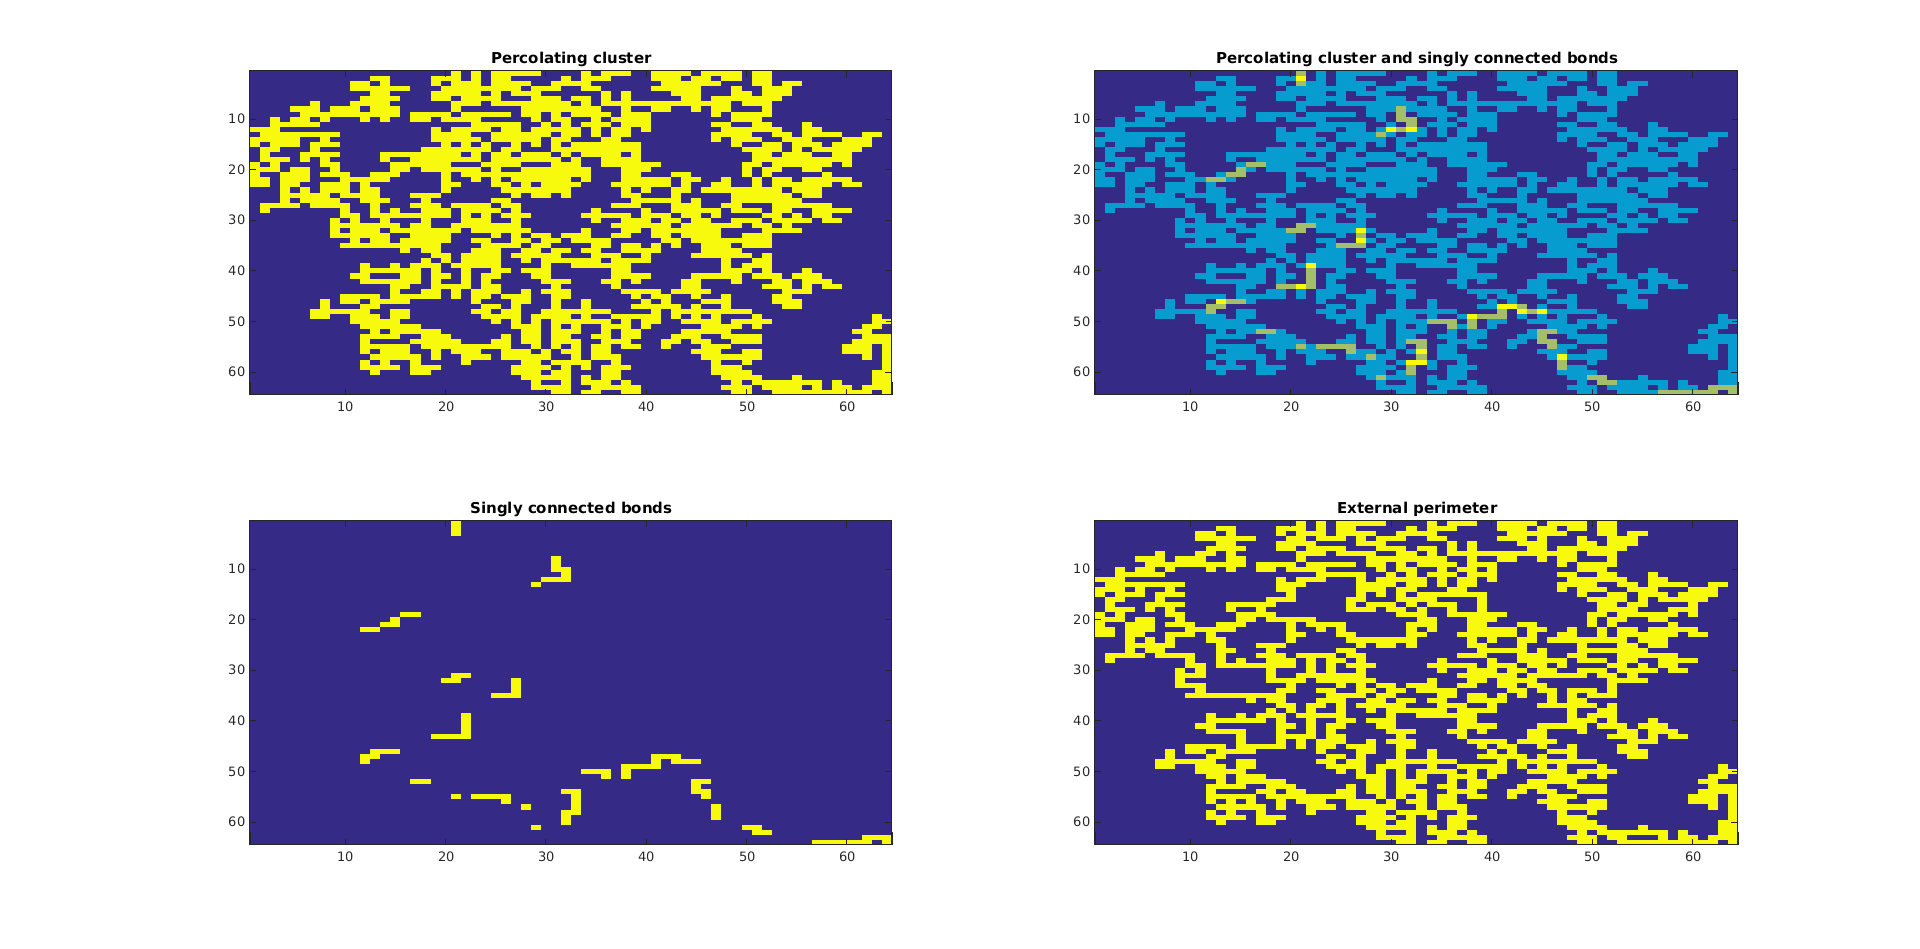
\includegraphics[width = 140mm]{../Figures/singlyConnectedBonds.png}
  \caption{SCB}
  \label{fig:fig11}
  \end{center}
\end{figure}


\subsection{ 19. Flow in a disordered system}
\textit{How do you measure the conductivity of the spanning cluster? Discuss the scaling theory
for the conductivity $\sigma(p,L)$ when $p > p_c$. Relate the results to permeability in a nanoporous
system.} \\

\noindent
\textit{Konduktivitet} $\sigma$ er en innebygd egenskap ved et materiale ved en gitt temperatur, hvor god 
ledningsevne materialet har. \textit{Konduktans} $G$ er avhengig av størrelsen og formen til materialet:
\begin{equation}
 G = \frac{L^{d-1}\sigma}{L} = L^{d-2}\sigma
\end{equation}
altså prop med tverrsnittsarealet og omvendt prop. med lengden. Volumfluksen er gitt ved Darcys lov, som 
for det nanoporøse systemet ovenfor:
\begin{equation}
 \Phi = \frac{kA}{\mu L}\Delta p = L^{d-2}\frac{k}{\mu}\Delta p = G\Delta p
\end{equation}
altså er konduktansen prop.konstanten for fluksen og trykkforskjellen, jfr. Ohms lov. 
Konduktiviteten er $\sigma = k/\mu$. For et perkolasjonssystem $L^d$, har vi at konduktansen er 1
for bonds mellom okkuperte sites, og 0 for ikke-okkuperte bonds. Vi finner $G$ ved å måle
total fluks ved en gitt trykkforskjell over sample:
\begin{equation}
 G = \frac{\Delta p}{\Phi} = G(p,L)
\end{equation}
Distribusjonen av flukser er
\begin{equation}
 \phi_{i,j} = g_{i,j}(p_i - p_j)
\end{equation}
der $g_{i,j} = k_{i,j}a/\mu l$ er konduktansen mellom nabosites $i$ og $j$, $l$ er avst. mellom dem og 
$a$ er tverrsnittarealet til bindingen. I følge kontinuitetslikningen er total flukt i site $i$ summen
av fluks inn i site $i$ fra alle nabosites $j$:
\begin{equation}
 \Phi_i = \sum_j g_{i,j} (p_i - p_j)
\end{equation}
Dette kan summeres for alle sites $i$, men bare sites ved grensene vil ha $\Phi_i \neq 0$. Ved alle andre
sites vil det være like mye som strømmer inn som strømmer ut. Hvis man finner total fluks for systemet
kan man finne total konduktans $G$, og dermed også konduktiviteten 
\begin{equation}
 \sigma = GL^{-(d-2)}
\end{equation}
MEN HVORDAN INDUSERER VI FLOW OVER PERKOLASJONSCLUSTER????

\subsubsection{Skalering av konduktivitet}
For et uendelig system må vi tar for oss konduktivitet, ikke konduktans. 
Simuleringer har vist at $P \propto (p-p_c)^\beta$ når $p\to p_c$, der $\beta > 1$. 
Konduktiviteten derimot, har en slakere kurve: $\sigma \propto  (p - p_c)^\mu$ der $\mu < 1$. 
Dette forklares ved at dangling ends ikke bidrar til konduktivitet, kun backbone, og vi har 
\begin{equation}
 D_B < D
\end{equation}
Vi tar nå for oss et system der $p > p_c$ og $L \gg \xi$. Ved lengdeskalaer større enn $\xi$ vil systemet
her være homogent (vi vil ha små clusters jevnt distribuert over en stor lengdeskala). Vi kan dele systemet
inn i bokser av størrelse $\xi$. For et homogent system har vi derfor at konduktansen er
\begin{equation}
  G(\xi,L) = (L/\xi)^{d-2}G(\xi,\xi)
\end{equation}
hvor $G(\xi,\xi)$ er konduktiviteten i en boks, der vi har $L \propto \xi$. Konduktiviteten er da
\begin{equation}
 \sigma(\xi,L) = L^{-(d-2)}G(\xi,L) = \frac{G(\xi,\xi)}{\xi^{d-2}}
\end{equation}
$G(\xi,\xi)$ kan tolkes som konduktansen til spanning cluster ved $p=p_c$ fordi et system med $L=\xi$ er identisk 
med et system ved $p = p_c$. Når $L \ll \xi$ oppfører systemet seg som om det er ved perkolasjonsterskelen, med 
en uendelig korrelasjonslengde, derfor $G = G(\infty,L)$. Vi har at
\begin{equation}
 G(\infty,L) \propto L^{-\tilde{\zeta}_R}
\end{equation}
der vi har kan vise ved resistivitetsargumenter at
\begin{equation}
 D_{SC} \leq \tilde{\zeta}_R \leq D_{min}
\end{equation}
Dette kan vi bruke til å få en skalering av $G$ ved systemstørrelse $\xi$:
\begin{equation}
 G(\xi,\xi) \propto \xi^{-\tilde{\zeta}_R}
\end{equation}
For $p > p_c$ har vi da at
\begin{equation}
 \sigma \propto \frac{G(\xi,xi)}{\xi^{d-2}} \propto \xi^{-(d-2+\tilde{\zeta}_R)}
 \propto (p-p_c)^{\nu(d-2+\tilde{\zeta}_R)} \propto (p-p_c)^\mu
\end{equation}
der $\mu = \nu(d - 2 + \tilde{\zeta}_R)$. Vi ser at for alle verdier $\tilde{\zeta}_R > 1/\nu$ så har vi 
for $d=2$ at $\mu > 1$ som nevnt ovenfor. 















 

\end{document}



\begin{comment}

% deloppgave
\begin{enumerate}
\item[\bf a)]
\item[\bf b)]
\item[\bf c)]
\item[\bf d)]
\end{enumerate}

%%%%%%%%
% Tabell
\begin{table}[H]
  \centering
  \begin{tabular}{ | c | r | r | r | r | r |}
    \hline
    & & & & & \\*
    \hline
    & & & & & \\*
    \hline
  \end{tabular}
  \caption{some caption}
  \label{tab:Tabell1}
\end{table}

%%%%%%%%
% Enkel figur
\begin{figure}[H]
\begin{center}
  \includegraphics[width = 120mm]{/users/filiphl/Desktop/Studie/Emne/ObligX/filnavn.png}
  \caption{some caption}\label{fig:fig1}
  \end{center}
\end{figure}

%%%%%%%%
% 2 figurer sbs
\begin{figure}
\begin{minipage}[t]{0.48\linewidth}
  \includegraphics[width=\textwidth]{fil}
  \caption{}
  \label{fig:minipage1}
\end{minipage}
\quad
\begin{minipage}[t]{0.48\linewidth}
\includegraphics[width=\textwidth]{fil}
  \caption{}
  \label{fig:minipage1}
\end{minipage}
\end{figure}

%%%%%%%%
% X antall kollonner
\begin{multicols*}{X}
\begin{spacing}{0.7} % verticale mellomrom
%kan f.eks benytte align?
\end{spacing}
\end{multicols*}


%%%%%%%%
%Matrise
\begin{equation*}
    {\bf A} = \left(\begin{array}{cccccc}
                           z &z &z &z &z &z \\
                           z &z &z &z &z &z \\
                           z &z &z &z &z &z \\
                           z &z &z &z &z &z \\
                           z &z &z &z &z &z \\
                           z &z &z &z &z &z \\
                      \end{array} \right)
\end{equation*}
%%%%%%%%

\end{comment}